\chapter{Discussion}\label{chapter:discussion}

Fundamental properties of M-dwarfs in eclipsing binary systems is a fast progressing field in which new measurements are published frequently. I am aware that new measurements are currently being prepared and may be published during the writing of this work. Currently there are four instalments of the EBLM project; I have submitted the fifth instalment of the EBLM project to Astronomy \& Astrophysics (five EBLMs observed with ground-based instruments) which is currently under review. The sixth instalment, authored by my collaborators, contains nine EBLMs which are not discussed here; this work has also been submitted and is under review. It is my intention to publish the four EBLM systems observed with K2 as the seventh instalment of the EBLM project in fore-coming months. 
%The first data release from TESS is anitcipated, but measurements from Gaia DR2 are included in this work. 
 To avoid re-writing this discussion numerous times, I will only discuss results published prior to 1$^{\rm st}$ September 2018.  


%%%%%%%%%%%%%%%%%%%%%%%%%%%%%%%%%%%%%%%%%%%%%%%%%%%%%%%%%%%%%%%%%%%%%%%%%%%%%%%%%%%%%%%%%%
%
%                          THE MASS RADIUS DIAGRAM
%
%%%%%%%%%%%%%%%%%%%%%%%%%%%%%%%%%%%%%%%%%%%%%%%%%%%%%%%%%%%%%%%%%%%%%%%%%%%%%%%%%%%%%%%%%%
\section{The mass-radius diagram}\label{discuss:mass-radius}

\begin{figure}
    \centering
    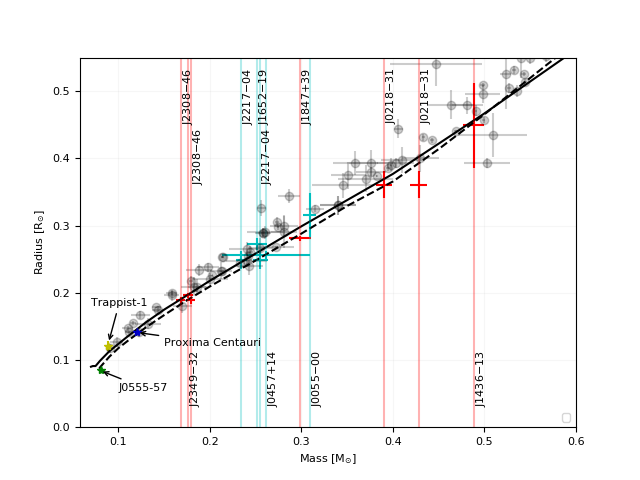
\includegraphics{9-Discussion/images/mass_radius.png}
    \caption{The mass and radius of 5 EBLMs from ground-based data (red) and 4 EBLMs observed with K2 (blue). We plot low-mass M-dwarfs with masses and radii known to better than 10\% (from Table 4 of \protect\citep{2018arXiv180505841C} and references therein). For J2308$-$46, J0218$-$31 and J2217$-$04 I plot both solutions and label accordingly. We also plot TRAPPIST-1 \protect\citep{2018MNRAS.475.3577D}, Proxima Centauri \protect\citep{2016Natur.536..437A} and J0555$-$57 \protect\citep{vonBoetticher2017}. }
    \label{discussion:fig:mass_radius}
\end{figure}

%The masses of the both stars for each EBLM were measured using \textsc{garstec} evolutionary models. The masses were then combined with the orbital solution to determine the radii of the M-dwarf companion. 

In Fig. \ref{discussion:fig:mass_radius}, I plot the 5\,Gyr isochrones for [Fe/H]$=0$\,dex (B15; \citealt{2015A&A...577A..42B}) and [Fe/H]$=-0.5$\,dex (B98; \citealt{1998A&A...337..403B}) and compare them to the nine EBLMs measured in this work. The B15 isochrones account for some of the flaws in the models presented by \citet{1998A&A...337..403B} (e.g. optical colours that are too blue). Visual inspection of the radii shows that they are broadly consistent with evolutionary models. The ground-based sample (red markers in Fig. \ref{discussion:fig:mass_radius}) have a sub-solar metalicity and are expected to have a radii between the B98 and B15 models. The K2 sample (cyan markers in Fig. \ref{discussion:fig:mass_radius}) have supersolar metallicity and are expected to lie above the B15 isochrone.

Three EBLMs (J0218$-$31, J1436$-$13 and J0055$-$00) have high impact parameters leading to a larger uncertainty in $R_\star / a$, $k$ and ultimately $R_1$ and $R_2$. The effect is most significant in J1436$-$13 and J0055$-$00 where the uncertainties in $R_2$ span across both B98 and B15 isochrones. The primary stars of five EBLMs (J2308$-$46, J0218$-$31, J0055$-$00, J1652$-$19 and J2217$-$04) have evolved into the ``blue-hook'' part of their post main-sequence evolution, leading to two solutions of$M_\star$, $M_2$ and $\tau$. Two of these systems (J0055$-$00 and J1652$-$19) have a single solution that is significantly favoured. The remaining three systems have solutions which hare only marginally favoured and so I report both in Tables. \ref{EBLMV_orb} \& \ref{EBLMVII_orb} and Fig. \ref{discussion:fig:mass_radius} as a precaution.
%Both solutions of J2217$-$04 and J2308$-$46 have radii which is positioned on the B95 and B15 isochrones. The older solution of J0218$-$31 is consistent with both B95 and B15 isochrones, but the moderately favoured younger solution is appears deflated by over 1-$\sigma$.



%%%%%%%%%%%%%%%%%%%%%%%%%%%%%%%%%%%%%%%%%%%%%%%%%%%%%%%%%%%%%%%%%%%%%%%%%%%%%%%%%%%%%%%%%%
%
%                           INFLATION AGAINST MESA
%
%%%%%%%%%%%%%%%%%%%%%%%%%%%%%%%%%%%%%%%%%%%%%%%%%%%%%%%%%%%%%%%%%%%%%%%%%%%%%%%%%%%%%%%%%%
\section{Bayesian measurements of radius inflation}\label{discuss:inflation}

The traditional approach of interpolating between solar B98 ([Fe/H] = 0) B15 ([Fe/H] = -0.5) isochrones of fixed age is not sufficient to assess inflation, especially for young systems below $1\,$Gyr which may still be contracting (e.g. J0457$+$14). A recent and well-sampled set of isochrones for low-mass stars are required to assess if the M-dwarf in each EBLM system is consistent with the isochrone for the respective measurement of [Fe/H] and $\tau$. For this task, I used the MESA isochrones. The MESA isochrones are created using the protosolar abundances recommended by \citet{2009ARA&A..47..481A} as the reference scale for all metallicities; this is consistent with the grid of spectra from wavelet analysis (Chapter \ref{chapter:wavelet}). MESA uses the OPAL equation of state tables from \citet{2002ApJ...576.1064R} along with opacity tables from \citet{2008ApJS..174..504F}, \citet{2011MNRAS.413.1828Y} and \citet{2010MolPh.108.2265F}. MESA also includes complex treatments for microscopic diffusion and gravitational settling (both important for low-mass stars), radiative levitation (important for high-mass stars), rotation, convective overshooting, magnetic fields and mass-loss. 

\begin{figure}
    \centering
    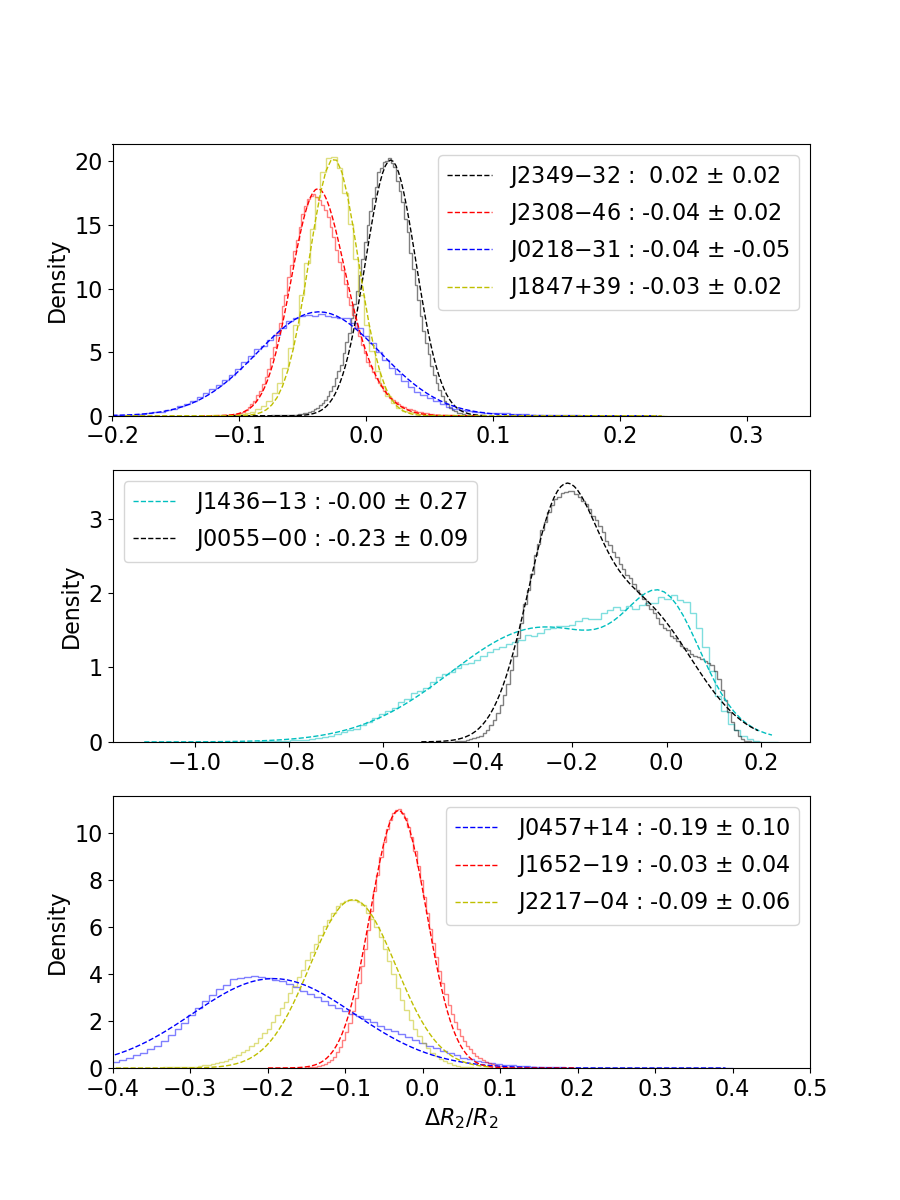
\includegraphics[width=0.9\textwidth]{9-Discussion/images/radius_inflation_EBLMs.png}
    \caption{The fractional radius residual PPD for each EBLM system. The middle panel has the two EBLMs that have broader PPDs which require a double Gaussian model. Of those that are better described by a single Gaussian model, EBLMs with follow-up photomtery from the ground are shown in the top panel, and those observed with K2 in the bottom panel. }
    \label{discussion:fig:radius_inflation}
\end{figure}

I used the web interpolater \footnote{http://waps.cfa.harvard.edu/MIST/interp\_isos.html} to create a grid of MESA isochrones  spanning the range [Fe/H]$=-2$ to $+0.5$\,dex in steps of\,0.5 dex and age range 0.8-9\,Gyrs in steps of 0.2 Gyrs. Using this grid, I created a bi-linear interpolation routine (in dimensions of $\tau$ and [Fe/H]) to obtain an expected radius, $R_{2,\rm exp}$ for a given mass. To assess inflation, the following procedure was employed for each draw in the PPDs from \textsc{eblmmass} and the orbital solution:

\begin{enumerate}
    \item $\log g_2$ can be calculated from the orbital solution using Eqn. \ref{suface_gravity}. 
    
    \item The corresponding draw for $M_2$ can be combined with $\log g_2$ to calculate the measured value of $R_2$,
    %
    \begin{equation}\label{r2_from_m2_and_g2}
        R_2 = \sqrt{\frac{G M_2}{g_2}}.
    \end{equation}
    %
    
    \item The corresponding draw for $\tau$ was used with a random number for [Fe/H] drawn from a Gaussian distribution of mean and width corresponding to the measurement of [Fe/H] and uncertainty of [Fe/H] reported in Table \ref{EBLMs_atmos} respectively to interpolate a MESA isochrone.
    
    \item The corresponding draw of $M_2$ was used to interpolate an expected radius for the M-dwarf companion, $R_{2, \rm exp}$. 
    
    \item $R_{2, \rm exp}$ and $R_2$ can be combined to calculate the fractional radius residual,
    %
    \begin{equation}
        \frac{\Delta R_2}{R_2} = \frac{R_2 - R_{2,exp}}{R_2}.
    \end{equation}
    %
\end{enumerate}

By repeating the above procedure for each step in the PPDs for \textsc{eblmass} and orbital fit, I was able to estimate the PPD for the fractional radius residual residual for each EBLM (Fig. \ref{discussion:fig:radius_inflation}). Four of the EBLMs with ground-based photometry along with three of those observed with K2 have narrow-peaked PPDs for $\Delta R_2 / R_2$ (top and bottom panel of Fig. \ref{discussion:fig:radius_inflation}). For these, I calculated the nominal fractional radius by binning the PPD into 100 bins and fitted a Gaussian model; I took the mean of the fitted Gaussian to be the measurement of $\Delta R_2 / R_2$ with uncertainty equal to the standard deviation. I found that a Gaussian shape is not a perfect fit to the PPDs of $\Delta R_2 / R_2$; there are asymmetric discrepancies where one side of the Gaussian model is lower than the PPD, whilst the other is too high. On average, the under-prediction on one side and over prediction on the other are of the same magnitude and I assume the widths still accurately represent the mean uncertainty of $\Delta R_2 / R_2$. The fitted models for J2308$-$46 and J0457$+$14 do not align well enough with the peak of the PPDs; the peak of the PPD was used as the measurement of $\Delta R_2 / R_2$ with the same uncertainty from the fitted model.

J0055$-$00 and J1436$-$13 have significantly higher impact parameters which broadens the PPD for $R_2$ and thus, $\Delta R_2 / R_2$ (middle panel of Fig. \ref{discussion:fig:radius_inflation}). I approximate this shape with a double Gaussian, and use an identical routine used to measure the double-peaked PPDs in Sect. \ref{methods:eblmmass}. The fit for J0055$-$00 is better than J1436$-$13. As a precaution, I used the peak of the PPDs for  J0055$-$00 and J1436$-$13 as the measurement of $\Delta R_2 / R_2$ with uncertainty equal to the standard deviations of each fitted Gaussian added in quadrature. 

The majority of systems appear deflated with respect to the MESA isochrones with no obvious differences between the top and bottom panels of Fig. \ref{discussion:fig:radius_inflation}. J2308$-$46, J0218$-$31 and J2217$-$04 have double-peaked distributions for $M_2$ and $\tau$ and I expected the PPDs for $\Delta R_2 / R_2$ to be shaped similar since $M_2$ is used to calculate $R_2$, and combined with $\tau$ to estimate $R_{\rm 2,exp}$. In creating the PPD for $R_2$ (Eqn \ref{r2_from_m2_and_g2}), the division of the PPD for $M_2$ with th PPD for $g_2$ diminishes the double-peaked nature observed in the PPD $M_2$, leading to a Cauchy-like PPD for $R_2$. The interpolated value of $R_{2, \rm exp}$ is dependent on $\tau$ and $M_2$ which are both double peaked. $R_{2, \rm exp}$ is not expected to have a double-peaked PPD as each combination of $\tau$ and $M_2$ was a trial step in \textsc{eblmmass} and will correspond to a similar expected radii (i.e. higher values of $\tau$ will correspond to lower values of $M_2$ and vice-versa). Thus the PPD for $\Delta R_2 / R_2$ is single peaked with width controlled by the uncertainty in $M_2$, $g_2$ and [Fe/H]. 










\subsection{Effect of stellar metalicity}

\begin{figure}
    \centering
    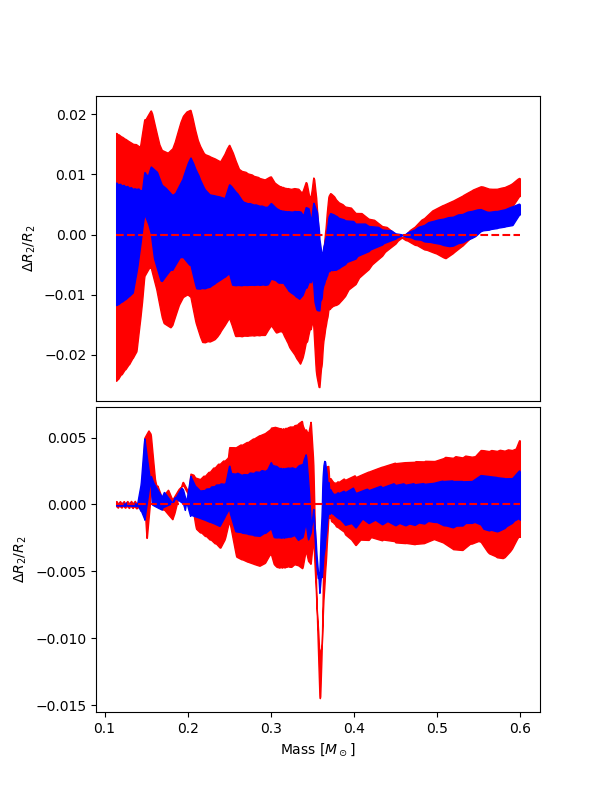
\includegraphics[scale=0.8]{9-Discussion/images/radius_sensitivity.png}
    \caption{The difference in fractional radius residuals of M-dwarfs from MESA evolutionary models relative to a 5\,Gyr isochrone with solar metallicity. (top panel) The difference in fractional radius residuals for an uncertainty of $\Delta$[Fe/H]$ = 0.06$ (blue) and $\Delta$[Fe/H]$ = 0.12$ (red) at a constant age of 5\,Gyr. (bottom panel) The difference in fractional radius residuals for an uncertainty of $\Delta \tau$ = 0.5\,Gyr (blue) and $\Delta \tau$ = 1\,Gyr (red) at [Fe/H]$ = 0$.}
    \label{fig:metalicity_diff}
\end{figure}


\begin{figure}
    \centering
    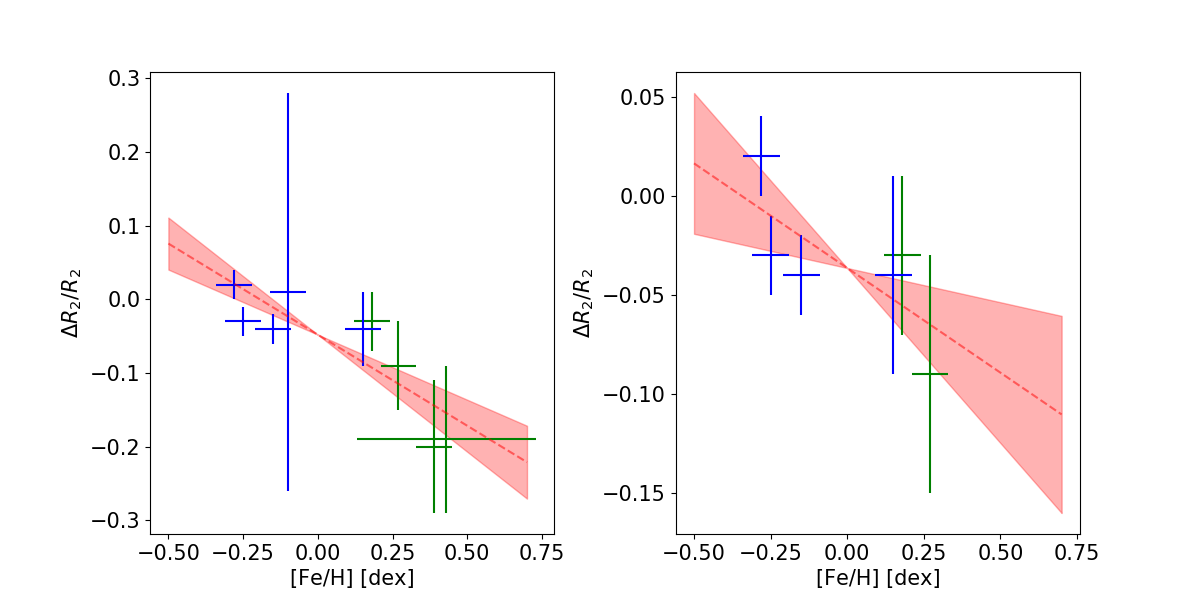
\includegraphics[width=\textwidth]{9-Discussion/images/inflation_with_metallicity.png}
    \caption{The fractional radius residual for all EBLMs measured in this work as a function of [Fe/H] (left panel). The same is also shown with J1436$-$13, J0055$-$00 and J0457$+$14 excluded (right panel). For each panel, we plot the best-fitting linear fit (red-dashed) with 1-$\sigma$ uncertainties in the gradiant (red fill).}
    \label{discussion:fig:metallicity_trend}
\end{figure}


Stellar metallicity directly affects the whole structure of a star. Most of the EBLMs have a metallicty uncertainty of 0.06\,dex (excluding J0457$+$14 and J1847$+$39). The uncertainty in metallicity changes the value of $R_{2, \rm exp}$, and thus increases the uncertainty in $\Delta R_2 / R_2$; this is visualised in the top panel of Fig. \ref{fig:metalicity_diff}. Although age dependent, I found the uncertainty in $\Delta R_2 / R_2$ increases between 0.005 and 0.015 depending on $M_2$. These uncertainties are comparable to the PPD widths of $\Delta R_2 / R_2$ for J2349$-$32, J2308$-$46 and J1847$+$39 and suggests that uncertainty in [Fe/H] is one of the dominant sources of uncertainty in $\Delta R_2 / R_2$ for EBLMs. Uncertainty in $\tau$ is typically between 0.13 - 1.78\,Gyr. In the bottom panel of Fig. \ref{fig:metalicity_diff}, an uncertainty of 5\,Gyr can lead to an uncertainty in $\Delta R_2 / R_2$ comparable with $\Delta \rm [Fe/H] = 0.06$\,dex for stars just below the convective transition. 


The metal content of M-dwarfs has been suggested to correlate with inflation (\citealt{2014ApJ...789...53F}; \citealt{2016A&A...593A..99F}; \citealt{2009A&A...505..205D}). 
%A study by \citet{2006ApJ...644..475B} found a positive correlation between radius inflation and [Fe/H] using six measurements of low-mass stars ($\leq\, 0.7 M_\odot$) with the CHARA array. The author suggests that this is caused by missing opacity sources which inflate the computed radii at high metallicity. Conversely, work by \citet{2013ApJ...779..183F} found a negative correlation with metallicity for detached eclipsing binaries ($M \leq\, 0.8\,M_\odot$ offering no explanation except that it is hinted in interferometric data of \citet{2012ApJ...757..112B}.  And finally, analysis of single stars which exclude the results of \citet{2006ApJ...644..475B} show little correlation with a single outlier at a large [Fe/H] that is not explained. This casts doubt that metallicity is the root cause of inflation for low-mass stars \citep{2009A&A...505..205D}.
The fractional radius residual of nine EBLMs presented in this work are plotted against [Fe/H] in Fig. \ref{discussion:fig:metallicity_trend}. There appears to be a negative correlation between [Fe/H] and $\Delta R_2 / R_2$ for all EBLMs (left panel of Fig. \ref{discussion:fig:metallicity_trend}). A Pearson correlation coefficient \citep{royal1895proceedings} is measured to be -0.84, indicating a strong, negative correlation between [Fe/H] and $\Delta R_2 / R_2$. A Pearson correlation coefficient may not be reliable for only nine data-points, but nevertheless aids the interpretation of any correlation. I fitted a $1^{\rm st}$-order polynomial to determine the best linear model using linear regression,
%
\begin{equation}
    \frac{\Delta R_2}{R_2} = (-0.247 \pm 0.071) \times \rm [Fe/H] - (0.048 \pm 0.019).
\end{equation}
%
I also fitted a 1-parameter model,  $\Delta R_2 / R_2 = c$, where $c = -0.065 \pm 0.001$. I compared both models using the Bayesian information criterion,
%
\begin{equation}
    BIC =  \chi^2 + k \log_e(n) ,
\end{equation}
%
where $k$ is the number of parameters for a given model and $n$ is the number of data points. If the standard error estimates for the data are reliable and the errors are normally distributed then the values of the $BIC$ can be used to compare models with different numbers of free parameters. In general, the model with the lowest BIC will give the optimum balance between the number of free parameters in the model and the goodness-of-fit. Assessing models can be done by calculating the difference in $BIC$ between the best model and the competing model. As a rule of thumb, a $\Delta BIC < 2$ means that neither model is favoured, $\Delta BIC = 2$--3 means that there is moderate evidence to suggest the model with the lowest $BIC$ is favoured and a $\Delta BIC > 6$ means that the evidence for the best model against the weaker model is strong. The linear and 1-parameter model have $BICs$ of 6.56 and 2.42 respectively, suggesting that the 1-parameter model is favoured. The $\Delta BIC = 4.41$ is moderate evidence to favour the 1-parameter model over the linear fit. 

Some of these EBLMs are not suitable to assess inflation. For example, the high impact parameters of J1436$-$13 and J0055$-$00 broaden the PPD for $\Delta R_2 / R_2$ to the extent in which they are no use for empirical calibrations or tests of evolutionary models. J0457$+$14 is a young, hot and fast rotating F-type star for which the M-dwarf companion's radius will still be contracting in the pre-main sequence. The uncertainty in  $\Delta R_2 / R_2$ for J0457$+$14 largely stems from an uncertain measurement of [Fe/H] as there are few measurable iron lines from which a reliable measurement of [Fe/H] can be obtained. We repeat these fits by excluding J1436$-$13, J0055$-$00 and J0457$+$14 (right panel of Fig. \ref{discussion:fig:metallicity_trend}). We find the best-fitting linear model,
%
\begin{equation}
    \frac{\Delta R_2}{R_2} = (-0.105 \pm 0.071) \rm [Fe/H] - (0.036 \pm 0.016),
\end{equation}
%
with a $BIC=10.35$. I tested for a 1-parameter model and found $c = -0.035 \pm 0.001$ with a $BIC = -4.48$ . A $\Delta BIC = 14.82$ is strong evidence to favour a 1-parameter fit. This suggests that trend with metallicity is statistically insignificant in both subsets; the absolute parameters of many more EBLMs are required to statistically assess any correlation between inflation and metallicity. 

The problem is somewhat complicated by the two different sources of EBLMs: those with ground-based follow-up photometry and those with observed with K2 (blue and green markers in Fig. \ref{discussion:fig:metallicity_trend}). Both groups had different lightcurve models, treatments of limb-darkening and red-noise models which may bias measurements of $\Delta R_2 / R_2$. The ground-based sample shows little evidence of any trend with [Fe/H] whilst the K2 sample appears to become increasingly deflated as metallicity increases. The validity of such conclusions is subject to interpretation as there is only a small sample size in each group.

If there are missing sources of opacity in the stellar models of low-mass stars, it may well be correlated with individual elemental abundances rather than [Fe/H] which implicitly assumes as metal scaling similar to the Sun. The grid of spectra used to measure the atmospheric parameters for these systems assumes solar abundances from \citet{2009ARA&A..47..481A}. I am the principle investigator of a SALT proposal (2017-1-SCI-041) to investigate if this is the case. I submitted a target list of 40 EBLM systems from \citet{Triaud2017} as a priority 4 proposal. In total, 30 were observed between $19^{th}$ May 2017 and $7^{th}$ August 2017 using SALT's high-resolution spectrograph (HRS) in medium resolution mode ($R \approx 37,000$). These observations were made in long slit mode with an exposure time scaling as a function of magnitude to ensure a SNR$\geq \, 100$. In future work, I will measure individual abundances for each spectra and look for correlations in with inflation. At the time of writing this thesis, only 4 of the 30 EBLMs that have been observed with SALT have reliable measurements of masses and radii. In future, TESS lightcurves in combination with more 1-m class telescope time will allow me test  this hypothesis.


\subsection{Orbital period and stellar radii}

%The inflation of M-dwarf radii is frequently associated with short orbital periods  (e.g. \citealt{2013ApJ...776...87S}). In tidally locked systems, M-dwarfs may be coerced into regimes of fast rotation which can enhance magnetic activity thus reducing convective efficiency leading to inflated radii \citep{2007A&A...472L..17C}. Enhanced magnetic fields affect the evolution of young low-mass stars which are still contracting onto the main sequence ($\leq\,1$\,Gyr); convective inhibition traps energy in their interiors, slowing contraction and leading to larger radii and cooler temperatures for a given age \citep{2016A&A...593A..99F}. The incorporation of magneto-convection into evolutionary models do predict surface magnetic fields $\sim 3\,kG$, which is consistent with X-ray luminosity estimates, and much larger interior fields to influence the structure of fully convective stars \citep{2013ApJ...779..183F}. Indeed, \citet{2013ApJ...779..183F} note that this is too strong to be stable and that a dynamo mechanism cannot produce such strong magnetic fields concluding they are unlikely to be responsible for inflating fully convective stars (see also \citealt{2016ApJ...818..189B}).

%A recent example is the red dwarf pair GJ65 AB \citep{2016A&A...593A.127K}. Components A \& B exceed radii expectations in the mass-radius plane by around 14\% and 12\%, respectively. This has been assumed to result from magnetic inhibition in both fast-rotating components. Their conclusion is strengthened when \citet{2016A&A...593A.127K} compare GJ65 to an almost identical, slow-rotating red-dwarf Proxima which shows no inflation to relative to models. However, this is a bold claim from the analysis of two systems and a much larger sample size is required.

%The presence of magnetic fields are directly linked to stellar activity, which in-turn can be measured by H-alpha emission. Work by \citet{2013ApJ...776...87S} found activity indicators were independent of radii discrepancy in both single and binary star systems which is consistent with interferometric measurements by \citet{2012ApJ...757..112B}. The SALT spectra I have obtained for 30 EBLMs cover H-alpha emission as well as the calcium H\&K lines (3969\,$\AA$ and 3934\,$\AA$, respectively) from which chromospheric activity indicators can be measured for the cooler host stars (spectral type $\sim$K; \citealt{2006PASP..118..617R}).  

\begin{figure}
    \centering
    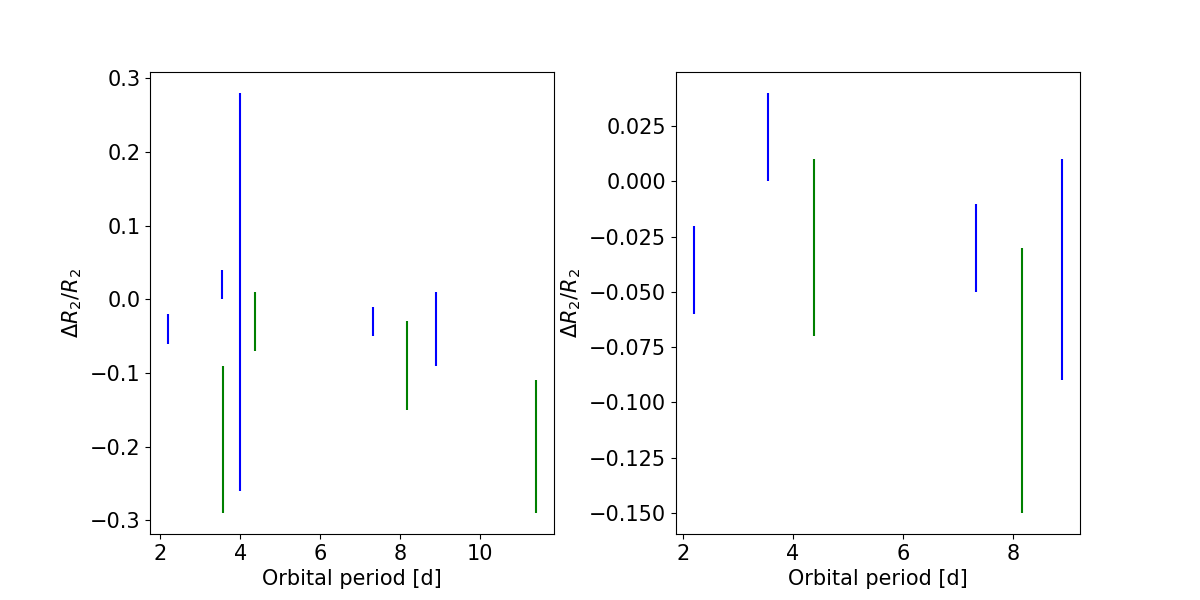
\includegraphics[width=\textwidth]{9-Discussion/images/inflation_with_period.png}
    \caption{The fractional radius residual for all EBLMs measured in this work as a function of orbital period (left panel). The same is also shown with J1436$-$13, J0055$-$00 and J0457$+$14 excluded (right panel).}
    \label{discussion:fig:inflation_with_period}
\end{figure}

EBLMs in tight orbits are more likely to be circularised and coerced into regimes of fast rotation. If this changes the magnetic structure of the M-dwarf leading to inflation, I would expect to see a clear link between orbital period and fractional radius residual. In Fig. \ref{discussion:fig:inflation_with_period}, I plot the fractional radius residual as a function of orbital period. There is no obvious correlations in Fig. \ref{discussion:fig:inflation_with_period}; Pearson correlation coefficients are -0.44 and -0.52 for the left and right panels respectively. This is suggests that there is a moderate negative correlation but is far from conclusive. The BICs for the 1-parameter fits are significantly lower than the linear counterpart ($\Delta BIC = 2.84$ and $2.12$ for the left and right panels of Fig. \ref{discussion:fig:inflation_with_period}) suggesting a 1-parameter model best describes the correlation between fractional radius residual and orbital period. I conclude that there is no clear correlation between inflation and orbital period for the nine EBLMs in this work.

%\begin{figure}
%    \centering
%    \includegraphics[width=\textwidth]{9-Discussion/images/inflation_%with_rot_period.png}
%    \caption{The fractional radius residual for all EBLMs measured in this work as a function of rotational period, for those that have measured rotational periods (left panel). The same is also shown with J1436$-$13 excluded (right panel).}
%    \label{discussion:fig:inflation_with_rot_period}
%\end{figure}

%Using the orbital period as a proxy for the rotational period assumes synchronisation which may not have occurred yet (see Sect. \ref{discuss:tidal}). For six EBLMs, we were able to make a tentative detection of rotational period from either WASP photometry, K2 photometry, or both. Two systems with ellipsoidal variation (J2308$-$46 and J0457$+$14) along with J0055$-$00 (where there is a possible detection of ellipsoidal variation) are the only systems which I could not estimate a rotational period. I plot the rotational period as a function of fractional radius residual in Fig. \ref{discussion:fig:inflation_with_rot_period}. Both panels in Fig. \ref{discussion:fig:inflation_with_rot_period} have a lower $BIC$ value for the 1-parameter fit compare to the linear fit ($\Delta BIC = 0.75$ and $\Delta BIC = 0.60$ for the left and right panels respectively) suggesting inflation is not correlated with rotational period either. EBLMs with orbital periods below 5\,d are likely to be influenced by tidal forces \citep{2005A&A...433L..21P} so I expected to see some significant difference of fractional residual radii with either side of a 5-d rotational/orbital period. 








%%%%%%%%%%%%%%%%%%%%%%%%%%%%%%%%%%%%%%%%%%%%%%%%%%%%%%%%%%%%%%%%%%%%%%%%%%%%%%%%%%%%%%%%%%
%
%           SECONDARY TEMPERATURE OF J0055-00
%
%%%%%%%%%%%%%%%%%%%%%%%%%%%%%%%%%%%%%%%%%%%%%%%%%%%%%%%%%%%%%%%%%%%%%%%%%%%%%%%%%%%%%%%%%%
\section{Temperature of the M-dwarf in J0055$-$00}\label{discuss:J0055-00T2}

\begin{figure}
    \centering
    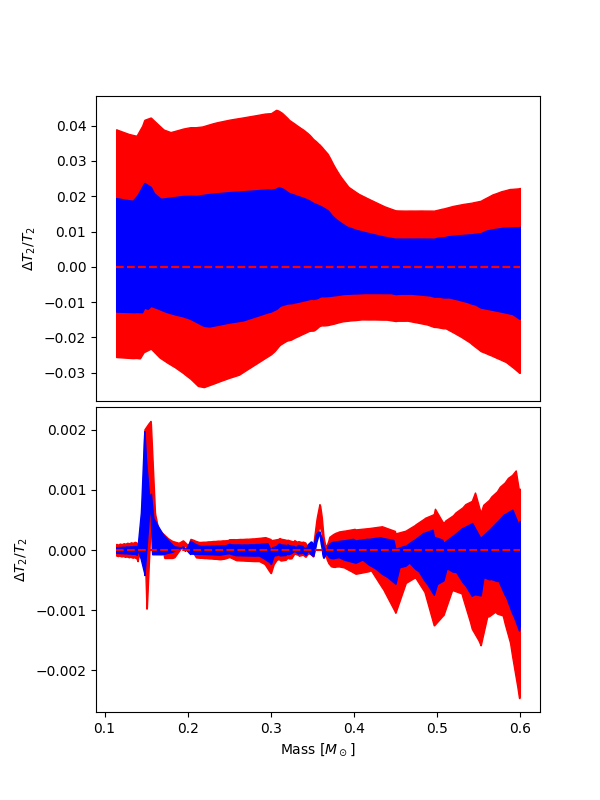
\includegraphics[scale=0.8]{9-Discussion/images/T2_sensitivity.png}
    \caption{The difference in fractional residuals of M-dwarfs temperatures from MESA evolutionary models relative to a 5\,Gyr isochrone with solar metallicity. (top panel) The difference in fractional radius residuals for an uncertainty of $\Delta$[Fe/H]$ = 0.06$ (blue) and $\Delta$[Fe/H]$ = 0.12$ (red) at a constant age of 5\,Gyr. (bottom panel) The difference in fractional residuals of M-dwarfs temperatures for an uncertainty of $\Delta \tau$ = 0.5\,Gyr (blue) and $\Delta \tau$ = 1\,Gyr (red) at [Fe/H]$ = 0$.}
    \label{fig:T2_diff}
\end{figure}

The effective temperature of the M-dwarf companion to J0055$-$00 is $\sim 510$\,K hotter than predicted by MESA isochrones. Similar observations have been observed for J0113$+$31 \citep{2014A&A...572A..50G} and KIC 1571511 \citep{2012MNRAS.423L...1O}. The temperature of an M-dwarf companion is sensitive to metallicity and age in a similar fashion to $\Delta R_2 / R_2$. (see Fig.\ref{fig:T2_diff}). Metalicity has an important effect on the fractional temperature residual,
%
\begin{equation}\label{discussion:relative_temperature}
    \frac{\Delta T_2}{T_2} = \frac{T_2 - T_{\rm 2,exp}}{T_2},
\end{equation}
%
across the M spectral type, with a more significant influence below 0.4\,$M_\odot$. Age changes the temperature between 1--2 orders of magnitude less than uncertainty in metallicity depending on which mass range is considered. Age uncertainty is likely to have a negligible contribution to the uncertainty of $\Delta T_2 / T_2$ ($\leq 0.2\%$) for main-sequence M-dwarfs, but may become important for younger systems below 0.5\,Gyr (i.e. J0457$+$14) where the surface temperature drastically reduces during pre-main sequence contraction. 

To assess the fractional temperature residual, I used a similar procedure to Sect. \ref{discuss:inflation} in combination with \textsc{pheonix} model spectra. For each draw in the PPDs from \textsc{eblmmass} and the orbital solution, the procedure was as follows:

\begin{enumerate}
    \item Random values of $T_{\rm eff}$, [Fe/H] and $\log g$ were generated from normal distributions using the mean as the measurements from Table.\ref{EBLMs_atmos} and the respective uncertainties as widths. These were be used to interpolate a \textsc{pheonix} model spectra for the primary star. 
    
    \item The same value of [Fe/H] with the corresponding draw for $\log g_2$ was used to continually interpolate spectra for a value of $T_{\rm 2}$ that matched the light ratio predicted in the K2 band-pass from the corresponding draw of $S$ and $k$ (until $\Delta S \leq 10^{-4}$).
    
    \item A \textsc{mesa} isochrone is interpolated using the same value of [Fe/H] with corresponding draw for $\tau$ and $M_2$, from which the expected temperature, $T_{\rm r,exp}$, is interpolated. 
    
    \item The value of $\Delta T_2 / T_2$ is calculated using Eqn. \ref{discussion:relative_temperature}.
\end{enumerate}

\begin{figure}
    \centering
    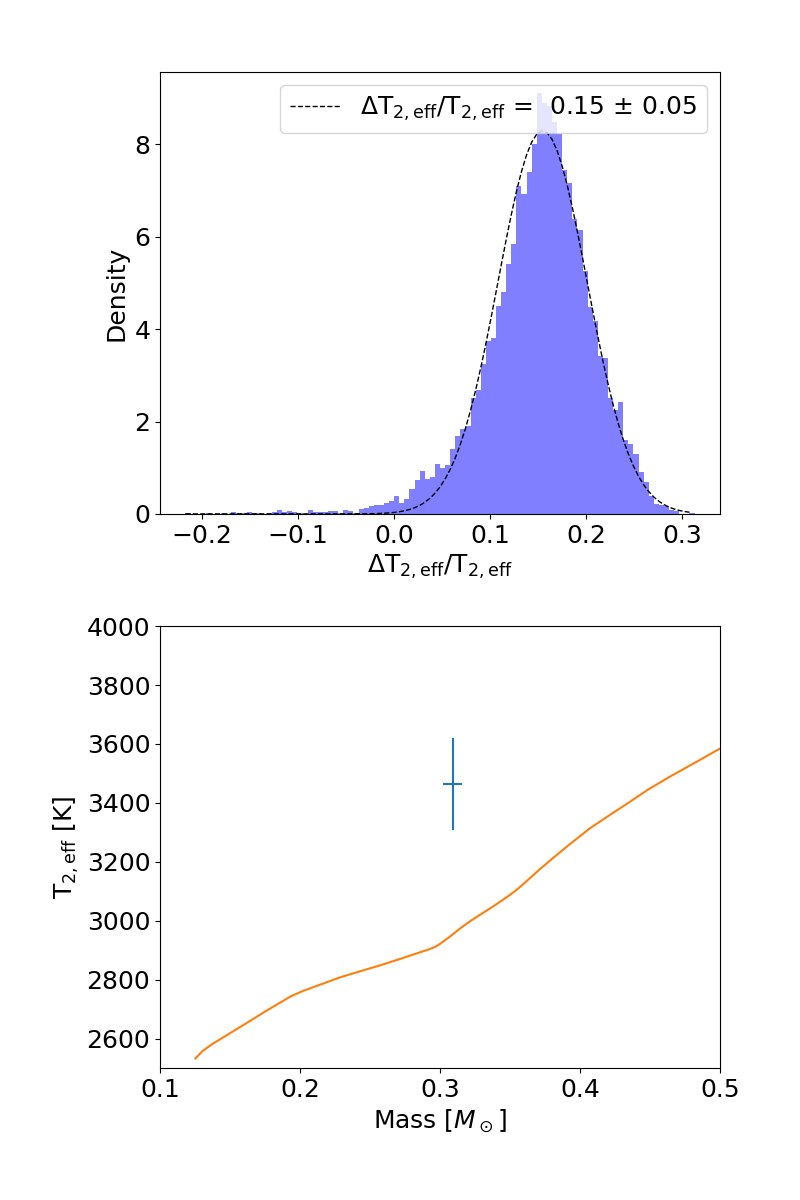
\includegraphics[scale = 0.6]{9-Discussion/images/T2_inflation.png}
    \caption{(top panel) The fractional temperature residual for the M-dwarf in J0055$-$00 (blue) with best-fitting Gaussian model (black-dashed). (bottom panel) The position of the M-dwarf in J0055$-$00 in the mass-temperature plane (blue) with best-fitting isochrone from \textsc{mesa}.}
    \label{discussion:fig:T2_inflation}
\end{figure}

The PPD for $\Delta T_2 / T_2$ for the M-dwarf companion in J0055$-$00 is shown in Fig. \ref{discussion:fig:T2_inflation}, along with it's position relative to the expected $M_2$-$T_{2}$ isochrone.  The PPD for $\Delta T_2 / T_2$ is shaped similarly to PPDs for $\Delta R_2 / R_2$; I fitted a Gaussian to the histogram (100 bins) and adopted the measurement of $\Delta R_2 / R_2$ to be the mean of the Gaussian with uncertainty equal to the width. I find that the temperature of M-dwarf is 3-$\sigma$ (~$510$\,K) hotter than what is expected from \textsc{mesa} isochrones. The discrepancy between measured and expected temperature is similar to temperature of the M-dwarf component for J0113$+$31 ($~ 600$\,K; \citealt{2014A&A...572A..50G}).  \citet{2014A&A...572A..50G} explore a variety of scenarios which may cause a temperature which is hotter than predicted. In the following sections, I explore these scenarios in the context of J0055$-$00.

\subsection{Model atmospheres}

I used the \textsc{pheonix} model atmospheres to estimate the effective temperature of the M-dwarf companion. As a self-consistency check, we interpolate \textsc{pheonix} spectra for the primary and M-dwarf star and convolved them with the K2 band-pass (accounting for $k$). \textsc{pheonix} models predict a drop in flux of 0.121\% for the secondary eclipse, which is consistent with observation. We interpolate the same spectra using Kurucz model spectra obtained through the \textsc{starlink} package \textsc{dispo} \citep{2014ascl.soft05016H}. Kurucz spectra predict a slightly more shallow drop in flux of 0.118\% but this is still consistent with the observed secondary eclipse depth.

\subsection{$\alpha_{\rm MLT}$, $\Delta Y$ and $l_3$}

In Sect. \ref{discuss:uncertainties}, I discussed the influence of $\alpha_{\rm MLT}$ and $\Delta Y$ in the context of uncertainty for $M_1$, $R_1$ and $\tau$. I fund that the additional uncertainty for $M_2$ and $\tau$  introduced by  $\Delta \alpha_{MLT} = 0.28$ and $\Delta Y = 0.02$ is 5\% and 1.5\,Gyr respectively. I re-determined  $\Delta T_2 / T_2$ for the M-dwarf companion in J0055$-$00 with errors in $M_2$ and $\tau$ inflated by 5\% and 1.5\,Gyr respectively. I found that the The PPD for $\Delta T_2 / T_2$ is broadened slightly, but is not enough to be consistent with evolutionary models.

\subsection{Metallicity offset}

The \textsc{mesa} evolutionary models use the same solar abundances from \citet{2009ARA&A..47..481A} as the grid used in wavelet analysis of CORALIE spectra and synthesis of spectra for INT observations. However, wavelet decomposition systematically underestimates [Fe/H] relative to \citet{Doyle2015}. I corrected the measurement of [Fe/H] for each EBLM using Eqn. \ref{composition_correction}. If I assume the original measurement of [Fe/H] was correct, the iron content of J0055$-$00 would be revised to [Fe/H]$=0.21 \pm 0.06$. Lowering the metallicity of the M-dwarf results in a higher surface temperature. I re-determined $\Delta T_2 / T_2 \approx 0.05$ using the aforementioned framework with the revised iron content. I found that the same PPD shape as Fig. \ref{discussion:fig:T2_inflation} with a fitted Gaussian indicating $\Delta T_2 / T_2 = 0.11 \pm 0.05$. This is 2-$\sigma$ too hot and so I conclude that the metallicity offset is not sufficient to account for the discrepancy in $T_{\rm 2,eff}$, although it may help to mitigate the problem.

\subsection{Contamination from unresolved components}

The presence of an unresolved background star or companion would affect the depth of the primary and secondary eclipses. The effect would be less for the primary eclipse than the secondary eclipse\footnote{If the wavelength of the data for the primary and secondary eclipses are very different, as in the case of \citet{2014A&A...572A..50G}.} due to the high luminosity ratio, except for cases with more exotic blends such as white dwarfs \citep{2014A&A...572A..50G}. A physically associated tertiary component may be observable with radial velocity measurements depending on the period of the orbit, RV sensitivity, orbital inclination, and observation time-span. Indeed, \citet{Triaud2017} found an EBLM tertiary rate of 17.8\% indicating that one or two systems in this sample should have a third-body in the system. For the case of J0055$-$00, I found that the value of $d(V_0) / dt$ is consistent with zero. However, J0055$-$00 was observed with CORALIE for just over one year, which may not be enough to detect an associated tertiary component that may have an orbital period of many years. I find no wavelength-dependent residuals in the SED fit which is good evidence to suggest that there is no unresolved component/background star contributing significantly different colours. There were no stars identified in Gaia DR2 other than J0055$-$00 within the K2 apertures. If there were, the excess flux would decrease the secondary eclipse transit depth, and thus the measured value of $T_2$.   



\subsection{Star spots}

Star spots on M-dwarfs have the effect of reducing the effective temperature and increasing the radius (e.g., \citealt{2007A&A...472L..17C}). The presence of spots on the M-dwarf would decrease the expected temperature from evolutionary models and decrease $\Delta T_2 / T_2$. The presence of hotspots on M-dwarfs is highly debated \citep{2014A&A...572A..50G} and we can't identify photometric variations which originate from the M-dwarf. Such a hot-spot need to be sufficient in size/coverage to increase the average surface temperature by 510\,K. 

A second effect works in the opposite direction. Assuming that the spots on the M-dwarf companion have no bearing on $R_2$ or luminosity, the measured value of $T_{\rm 2,eff}$ will be higher for a spotted star because the non-spotted parts of the photosphere have to be hotter to counteract the lost flux from the spots so that luminosity remains constant. Tho hot parts of the photosphere dominate the flux at optical wavelengths so the flux from the spots is missed because it is emitted outside the K2 band-pass.



\subsection{Irradiation}

If both components are in a synchronous, circularised and close-in orbit then one side of the M-dwarf will be constantly irradiated by the host star. The orbital eccentricity  of J0055$-$00 suggest a near-circularised orbit and is likely not synchronised. Further to this, J0055$-$00 has the largest orbital period of the sample, with a semi-major axis $a = 24.39 \pm 0.54\,R_\star$; only $\approx 0.001\%$ of the primary stars luminosity ($1.479 \times 10^{22}\, \RM W\,s^{-1}$) will be irradiated onto the surface of the M-dwarf. However, the required energy input to heat up the M-dwarf by 510\,K (assuming a constant radius) is on the order of $2.336 \times 10^{24}\,W$ meaning that even a conservative albedo of unity would not be sufficient to increase $T_2$ by 510\,K.


\subsection{Residual heat from formation}

The surface temperature of M-dwarfs remains approximately constant over it's main-sequence life. There is a possibility that the M-dwarf formed significantly after the primary star resulting in an M-dwarf that is still contracting towards the main sequence. In the first 10\,Myr, \textsc{mesa} models predict that a 0.309\,$M_\odot$ M-dwarf will cool from a surface temperature of 3400\,K to 3150\,K. A younger M-dwarf is unlikely for two reasons: (1) the radius of the M-dwarf would be significantly inflated and I find it consistent with the radius predicted with a 3.52\,Gyr \textsc{mesa} isochrone and (2) it is unlikely that each component in the EBLM system formed at significantly different times \citep{2003ApJ...584..853P}. 


\subsection{Mass transfer and/or accretion}

Both components of J0055$-$00 are well-detached and inside their respective Roche lobes. They are not interacting, not transferring mass between and there is no evidence of circumbinary or circumstellar disks. Furthermore,  episodic accretion is likely to end after a few Myrs \citep{2009ApJ...702L..27B} making such heating unlikely. 

\subsection{Tidal heating}

The orbital separation and lack of eccentricity means that there will be little tidal deformation. In the case of J0113$+$31 (of similar period to J0055$-$00) presented by \citet{2014A&A...572A..50G}, they find that the smallest M-dwarf rotation period with the lowest values of dissipation created a tidal energy input $~ \times 10^{21}$\,W. This is 3 orders of magnitude too small to account for the measured temperature of the M-dwarf. 





%%%%%%%%%%%%%%%%%%%%%%%%%%%%%%%%%%%%%%%%%%%%%%%%%%%%%%%%%%%%%%%%%%%%%%%%%%%%%%%%%%%%%%%%%%
%
%                           SYSTEMATIC EFFECTS
%
%%%%%%%%%%%%%%%%%%%%%%%%%%%%%%%%%%%%%%%%%%%%%%%%%%%%%%%%%%%%%%%%%%%%%%%%%%%%%%%%%%%%%%%%%%

\section{Systematic effects  on determining mass, radius and age}\label{discuss:uncertainties}

The following section was written for a recently submitted paper which concerns only the EBLMs with follow-up photometry from ground-based instruments (J2349$-$32, J2308$-$46, J0218$-$31, J1847$+$39 and J1436$+$13). Subsequently, all discussion in this section refers only to these systems.

One major issue remains with the method employed in this work and previous publications of the EBLM project: I am attempting to test evolutionary models of low-mass stars using the models of better-understood F-/G-dwarfs. This method is acceptable when the uncertainty propagated by stellar models for F-/G-stars are much smaller than the propagated uncertainties in radial velocity measurements and transit photometry. This is not necessarily the case for the data I have used in work since it is possible to measure some orbital parameters listed in Chapter \ref{chapter:results} to better than a 0.2\%. In the following sections, I explore some systematic sources of uncertainty arising from using evolutionary models to determine the primary star, along with the impact of unresolved blends and choice of limb-darkening. 



\begin{sidewaystable*}
\caption{The difference in mass and radius of the primary star ($\star$) and the secondary (2) for a variety of different scenarios. The measured values were subtracted from those in Table. \protect{\ref{EBLMV_orb}}. For J2308-46 and J0218-31, we only considered the most probable solution in this work. We separately re-fitted with 10\, \% third light ($l3$) and using the quadratic limb-darkening law over the Claret law ($ldy$) from which we re-measured only the radii of the stars in the systems. We also separately recalculate the masses of the stars in each system by changing mixing length parameter from $1.50$ to $1.78$ ($\alpha_{mlt}$) and a change in helium enhancement values from $0.00$ to $0.02$ ($\Delta Y$). We also show the mean of each column, $\bar{x}$, calculated with all values excluding those from J1436-13 (marked with an asterisk).}              % title of Table
\label{systematic_light_table}      % is used to refer this table in the text
\centering                                    % used for centering table
\begin{tabular}{c l l  l l l l l l l l l l l l l }          % centered columns (4 columns)
\hline\hline 
 & $\Delta R_{\star,\, l3}$ & 
 $\Delta R_{2,\, l3}$ 
 &$\Delta R_{\star,\, ldy}$ & 
 $\Delta R_{2,\, ldy}$ 
 
 & $\Delta M_{\star,\, \alpha_{mlt}}$
 & $\Delta M_{2,\, \alpha_{mlt}}$
 & $\Delta \tau_{\alpha_{mlt}}$

 & $\Delta M_{\star,\, Y}$
 & $\Delta M_{2,\, Y}$
 & $\Delta \tau_{Y}$



  \\
\hline

J2349-32 & $-0.002$ & $-0.016$ & $-0.014$ & $-0.002$ & $-0.037$ & $-0.004$ & $2.208$ & $0.048$ & $0.005$ & $-0.853$ & \\

J2308-46 & $-0.003$ & $-0.011$ & $-0.017$ & $-0.001$ & $-0.045$ & $-0.003$ & $1.703$ & $0.056$ & $0.004$ & $-1.201$ & \\

J0218-31 & $-0.007$ & $-0.012$ & $-0.005$ & $-0.002$ & $-0.057$ & $-0.001$ & $0.503$ & $0.041$ & $0.006$ & $-0.254$ \\

J1847+39 & $-0.008$ & $-0.016$ & $-0.015$ & $-0.004$ & $-0.046$ & $-0.001$ & $1.071$ & $0.052$ & $0.009$ &  $-0.820$ \\
	
J1436-13* & $-0.162$ & $-0.064$ & $-0.059$ & $-0.090$ & $-0.024$ & $-0.005$ & $-0.135$ & $0.043$ & $0.011$ & $-1.150$ \\


\hline 
$\bar{x}$ & $-0.005$ & $-0.013$ & $-0.012$ & $-0.003$ & $-0.046$ & $-0.002$  & $1.070$  & $0.050$ & $0.007$ & $0.855$  \\


\hline
\end{tabular}
\end{sidewaystable*}

%%%%%%%%%%%%%%%%%%%%%%%%%%%%%%%%%%%%%%%%%%%%%%%%
%    Evolution ambiguity, Y and alpha_mlt      %
%%%%%%%%%%%%%%%%%%%%%%%%%%%%%%%%%%%%%%%%%%%%%%%%
\subsection{Evolution ambiguity, $\alpha_{\rm MLT}$ and $Y_{\rm He}$}
%PFLM
The default model grid used in \textsc{eblmmass} uses a mixing length parameter $\alpha_{MLT} = 1.78$ and an initial helium abundance $\rm Y = 0.26646 + 0.984 \rm \,Z$, both of which have been calibrated on the Sun. As noted by \citet{2015A&A...575A..36M}, these assumptions are subject to some level of uncertainty.  \citet{2015A26A...577A..90M} estimated the uncertainty in mass, $M_{\star}$, and age, $\tau$, for 28 transiting exoplanet host stars by assuming an error of 0.2 in $\alpha_{MLT}$ and 0.02 for initial helium enhancement, $\Delta Y$ for each star. They found that systematic errors in mass and age from $Y$ and $\alpha_{MLT}$ can be comparable to the random errors in these values for typical observational uncertainties in the input parameters. The sample measured by \citet{2015A26A...577A..90M} consists primarily of stars less massive than the Sun, whereas the primary stars in this work are more massive F-type stars.  Three grids of models are provided with \textsc{eblmmass}: 1. $\alpha_{MLT} = 1.78$, $\Delta Y=0.00$, 2. $\alpha_{MLT} = 1.5$, $\Delta Y=0.00$ and 3. $\alpha_{MLT} = 1.78$, $\Delta Y=0.02$; I used grid 1 in Tables \ref{EBLMV_orb} \& \ref{EBLMVII_orb}. I re-measured the mass, radius and age of both components with the grids 2 and 3 to see how the uncertainties in $\alpha_{\rm MLT}$ and $\Delta Y$ impact our results. I used grid 2 to assess the impact of $\Delta \alpha_{MLT} = 0.28$ and grid 3 to assess the impact of $\Delta Y = 0.02$; I used the same orbital solution and atmospheric parameters from Chapter \ref{chapter:results}.


The mass uncertainties ($\Delta M_{\star}$ and $\Delta M_{\rm 2}$) in Table \ref{systematic_light_table} corresponding to $\Delta \alpha_{MLT} = 0.28$ are $ \approx 2-3 \%$, and are similar to those found by \citet{2015A26A...577A..90M}. Helium enhancement typically introduces a larger mass uncertainties $\approx 4-5 \%$. The opposite is seen for $\tau$ determinations, where a value of $\Delta \alpha_{MLT} = 0.28$ introduces an uncertainty of $1.07\, \rm Gyr$ and $\Delta Y = 0.02$ introduces an uncertainty of $\Delta \tau = 0.86\, \rm Gyr$. The typical uncertainty in $\tau$ from \textsc{eblmmass} for these EBLM systems is around $1\, \rm Gyr$ which can produce significant systematic offsets. The quadratic combination of uncertainty for $M_2$ introduced by $\alpha_{MLT}$ and $Y$ is around $0.01 \, M_{\odot}$ (3\% for a $0.4-M_{\odot}$ M-dwarf).

%A further limitation arises when the primary star enters te ``blue-hook'' part of t main-sequence evolution. Three host-stars in our sample (J2308$-$46, J0218$-$31 and J2217$-$04) are in this region leading to two distinct solutions for $M_{\star}$ and $\tau$. A single solution is preferred for all three systems but there will always be some ambiguity until further mass constraints can be obtained. Until then, these systems should not contribute to empirical calibrations. One approach for the EBLM project could be to pre-select cooler host stars ($\leq 6100$ K) to avoid host stars near the Henyey hook. Another solution may lie in the increased contrast between a host star and an M-dwarf in the infrared. It may be possible to detect molecular lines (VO, TiO, CaH, etc.) associated with an M-dwarf from using high-resolution infrared spectroscopy. This would enable radial velocity measurements of the secondary component, and turn the SB1 into an SB2, and place a further constraint on which mass and age solution best describes the system.

%%%%%%%%%%%%%%%%%%%%%%%%%%%%%%%%%%%%%%%%%%%%%%%%
%                 THIRD LIGHT                  %
%%%%%%%%%%%%%%%%%%%%%%%%%%%%%%%%%%%%%%%%%%%%%%%%

\subsection{Third light effect}\label{third_light_effect}



\begin{table*}
\caption{Distance measurements from Gaia DR2. We also report the orbital separation corresponding to an sky-projected separation of 0.3" for each EBLM system and the orbital period associated with this separation using $M_{\star}$ from Table \ref{EBLMV_orb}.}              % title of Table
\label{EBLM_seperation}      % is used to refer this table in the text
\centering                                      % used for centering table
\begin{tabular}{c c c c c}          % centered columns (5 columns)
\hline\hline                        % inserts double horizontal lines
EBLM & Parallax [$mas$] & d [$pc$] & Orbital separation at 0.3" [$au$] & Period  [$yr$] \\    % table heading
\hline                                   % inserts single horizontal line
    J2349-32 & $3.85 \pm 0.04$ & $259.69 \pm 2.83$   & $389 \pm 4$    &  $19.81 \pm 0.10$ \\      
    J2308-46 & $2.27 \pm 0.08$ & $440.78 \pm 15.19$  & $661 \pm 23$   &  $23.49 \pm 0.41$ \\
    J0218-31 & $3.84 \pm 0.04$ & $260.13 \pm 2.85$   & $390 \pm 4$    &  $15.86 \pm 0.08$ \\
    J1847+39 & $3.67 \pm 0.03$ & $272.83 \pm 1.89$   & $409 \pm 3$    &  $19.70 \pm 0.07$ \\
    J1436-13 & $2.15 \pm 0.05$ & $466.27 \pm 11.15$  & $699 \pm 16$   &  $24.29 \pm 0.28$ \\
\hline                                             %inserts single line
\end{tabular}
\end{table*}

The fits to the transit photometry in this work assumes zero light from the M-dwarf companion. Using the \textsc{phoenix} models of stellar evolution and Bessel filters we expect around 0.07\% of the total flux in the $R$ filter will be from the M-dwarf, with slightly more in the $I$ filter. I re-fitted J2349$-$32 with 0.07\% third light and measured a negligble change in $k$ and $R_\star / a$. Spectroscopy shows no contamination $>30\%$ (approximated from the quality of the spectrum) but we are insensitive to unresolved background or nearby stars providing $5-30\%$ third-light. Neglecting this will introduce addition uncertainty in radii measurements if not properly accounted for.  

Lucky imaging provides constraints on nearby contaminating objects. For J2349$-$32 and J2308$-$46, we find that the close companions do not significantly contaminate follow-up photometry. For J0218$-$31 and J1847$+$39 we can put constraints on the amount of third light from the consistency between the ratio of the radii measured from transit photometry in different pass-bands. For J1436$-$13 we have to rely on existing surveys to identify any nearby stars which may contaminate follow-up photometry.    Ground-based Lucky imaging has a upper-limit to resolve companions with a sky-projected separation of $\sim$0.3". The orbital separation for each EBLM corresponding to a sky-projected separation of 0.3" was calculated using parallax measurements from Gaia DR2 (Table \ref{EBLM_seperation}). The period of such orbits were also calculated using measurements of $M_{\star}$ from Table \ref{EBLMV_orb}. We find that the closest EBLM (J2349$-$32 at a distance of $259 \pm 3\, \rm pc$) would require a semi-major axis of at least $389\, \rm au$ with orbital period spanning two decades. The three-body systems identified by  \citet{Triaud2017} will have orbital periods on the order of decades and would be difficult or impossible to resolve through lucky imaging. 

The spectrum itself can provide useful constraints on potential aperture contamination. The analysis of CORALIE spectra for 118 EBLM systems presented by \citet{Triaud2017} found that 17.8\,\% of these systems show significant evident for non-zero values of $d(\gamma)/dt$ (spanning $d(\gamma)/dt = 0.07$ - 4.5 $\rm km\, \rm s^{-1}\, \rm yr^{-1}$). J0218$-$31 and J1847$+$39 have best-fitting values of $d(\gamma)/dt$ which are at the bottom of this bracket.  If these drifts are evidence of a third body, they would have separations which are challenging to resolve with lucky imaging and require decades of spectroscopic observations to characterise. The low SNR spectra from CORALIE and INT eliminates unresolved blends which contribute more than 30\% of the total system luminosity of the primary star by inspection of cross-correlation functions This eliminates the presence any bright companion or  back-ground star but ultimately means we cannot rule out unresolved objects which contribute $<30\,\%$ of the total luminosity. The transiting M-dwarf companions would contribute between 0.1\% - 15\% of the total luminosity and would be lost in the noise.

Including third light as a free parameter in the orbital fit will change the shape and depth of a light-curve and lead to a degeneracy between $R_{\star}$, $k$ and $b$.  I assessed this by re-fitting the orbital solution for all stars assuming a 10\% light contamination from a third body which does not interact with the EBLM system. From this fit, we combine best fitting values of  $R_{\star}/a$, $b$, and $k$ and their uncertainties with nominal values from the original fit to re-determine $R_{\star}$ and $R_{2}$ from \textsc{eblmmass} (first two columns in Table \ref{systematic_light_table}). On average, I found a 3-7\% increase in $R_2$ when third light is fixed to 10\,\%; with the largest uncertainty for the smallest M-dwarfs. I ignore J1436$-$13 from this discussion since the impact parameter is too high to draw meaningful conclusions about changes in measured radi. This is comparable to the inflation in radius for low-mass stars typically quoted in the literature (e.g.  3-5\%; \citealt{2013ApJ...776...87S}). However, if we were to see radius inflation in general for the M-dwarf components of EBLM systems then the third-light effect can only be a partial explanation. This is because the majority of these systems do not have detected third bodies in the system, and the third body will often contribute much less than 10\% of the total flux in these triple-star systems. 

%%%%%%%%%%%%%%%%%%%%%%%%%%%%%%%%%%%%%%%%%%%%%%%%
%                 LIMB DARKENING               %
%%%%%%%%%%%%%%%%%%%%%%%%%%%%%%%%%%%%%%%%%%%%%%%%


\subsection{Limb darkening}\label{limb_darkening_section}

\begin{table*}
\caption{Theoretical (marked with an asterisk) and fitted quadratic limb-darkening coefficients for  $a_1$ and $a_2$ using Eqn. \ref{quad_limb_law}.}              % title of Table
\label{quadratic_limb_darkening__table}      % is used to refer this table in the text
\centering                                    % used for centering table
\begin{tabular}{c c c c c c}          % centered columns (4 columns)
\hline\hline 
EBLM   & Filter& $a_1^*$ & $a_1$ & $a_2^*$ & $a_2$ \\
\hline

J2349-32  & I & $0.368 \pm 0.050$  & $0.400 \pm 0.010$ & $0.147 \pm 0.051$ & $0.145 \pm 0.050$    \\


J2308-46 & R & $0.460 \pm 0.050$ & $0.444 \pm 0.031$ & $0.150 \pm 0.051$ & $0.128 \pm 0.043$ \\

J0218-31 & g' & $0.718 \pm 0.051$ & $0.735 \pm 0.022$ & $0.050 \pm 0.052$ & $0.278 \pm 0.013$\\
&          r' & $0.508 \pm 0.050$ & $0.588 \pm 0.012$ & $0.136 \pm 0.052$ & $0.203 \pm 0.015$\\
&          i' & $0.412 \pm 0.050$ & $0.461 \pm 0.011$ & $0.143 \pm 0.051$ & $0.227 \pm 0.014$ \\
&          z' & $0.338 \pm 0.050$ & $0.341 \pm 0.009$ & $0.146 \pm 0.051$ & $0.201 \pm 0.015$\\

J1847+39 & CBB & $0.468 \pm 0.050$ & $0.461 \pm 0.034$ & $0.147 \pm 0.051$ & $0.217 \pm 0.015$ \\
&          g'  & $0.659 \pm 0.051$ & $0.631 \pm 0.057$ & $0.100 \pm 0.051$ & $0.223 \pm 0.015$ \\
&		   z'  & $0.303 \pm 0.050$ & $0.255 \pm 0.035$ & $0.214 \pm 0.050$ & $0.215 \pm 0.022$\\
	
J1436-13 & R & $0.453 \pm 0.050$ & $0.547 \pm 0.010$ & $0.151 \pm 0.051$ & $0.247 \pm 0.015$\\

\hline
\end{tabular}
\end{table*}

To determine accurate estimates for $R_{\star}$, $k$ and $b$ I required an accurate prescription for limb-darkening in our light curve model.  To fit the lightcurve for five EBLM systems observed from ground-based instruments, I used the Claret 4-parameter law \citep{Claret2000},
%
\begin{equation}\label{claret_limb_law}
\frac{I_\mu}{I_0} = 1 - \sum_{i =1}^{4} a_i(1-\mu^{\frac{1}{2}}_i),
\end{equation}
%
where $a_i$ is the $i^{th}$ limb-darkening coefficient and $\mu = \cos \gamma$, $\gamma$ being the angle between a line normal to the stellar surface and the line of sight to the observer. The coefficient tables I used to interpolate values of $a_i$ are described in Sect. \ref{method:orbital_fit}, and are interpolated for a given $T_{\rm eff}$, [Fe/H] and $\log g$. As described in Sect. \ref{method:orbital_fit}, I allowed the limb-darkening temperature, $T_{\rm eff, ld}$, to vary as a free parameter with a Gaussian prior from spectroscopy, and fix $\log g$ and [Fe/H] to values from wavelet analysis. An alternative is to use the quadratic limb-darkening law \citep{1950HarCi.454....1K} with only 2 parameters,
%
\begin{equation}\label{quad_limb_law}
\frac{I_u}{I_0} = 1 - \sum_{i =1}^{2} a_i (1 - \mu)^i.
\end{equation}
%
I assessed the impact of our choice of limb-darkening law on $R_{\star}$ and $R_2$ by re-fitting the five EBLMs observed with ground-based instruments using the quadratic limb darkening law (Eqn. \ref{quad_limb_law}). We generate coefficients $a_1$ and $a_2$ for each pass-band using the Python package \textsc{ldtk} (see Table \ref{quadratic_limb_darkening__table}; \citealt{Parviainen2015}). \textsc{ldtk} uses uncertainties from $T_{\rm eff}$, [Fe/H] and $\log g$ to estimate uncertainties in the calculated values of $a_1$ and $a_2$ ($\sigma_{a_1}$ and $\sigma_{a_2}$). I then used these uncertainties to apply Gaussian priors to $a_1$ and $a_2$ and stop the sampler tending to unrealistic values; the priors have a mean value and width calculated from \textsc{ldtk}. Errors on $a_1$ and $a_2$ from errors on $T_{\rm eff}$, etc. are very small and unlikely to reflect real uncertainty due to uncertainties in the models so I add a subjective value of 0.05 in quadrature to the uncertainties on each parameter to allow for this. A new combined orbit and light curve solution was found using the same number of draws used in Sect. \ref{method:orbital_fit}. From this solution, we use $R_{\star}/a$, $k$ and $b$ with their uncertainties and combine it with the orbital solution found in Chapter \ref{chapter:results} to measure the radii of components in each system. This ensures that only parameters relating to the radii of the stars were changed. 


I found that the uncertainty introduced by choice of limb-darkening law (Table \ref{quadratic_limb_darkening__table}) is less than introduced by third light. The primary and secondary stars see a similar reduction in $R_{\star}$ and $R_2$ between $0.5-2\%$; the largest uncertainty is attributed to the smallest stars for primary or secondary stars. \citet{2013A&A...549A...9C}, from their study of  exoplanet-host stars conclude that fixing the limb-darkening coefficients to theoretical values does not allow the determination of $R_2$ to better than $1$-$10 \%$; a reason why we fitted $a_1$ \& $a_2$. Intertwined in this are the effects caused by stellar activity, spots and faculae. These are time-dependent effects which change at each transit event and can modify the limb-darkening values far from what is predicted. One conclusion from \citet{2013A&A...549A...9C} is that a star with 0.5\% spot coverage can introduce a 1\% uncertainty on $k$.




\section{Tidal evolution}\label{discuss:tidal}
% https://arxiv.org/pdf/0908.2624.pdf


\begin{figure}
    \centering
    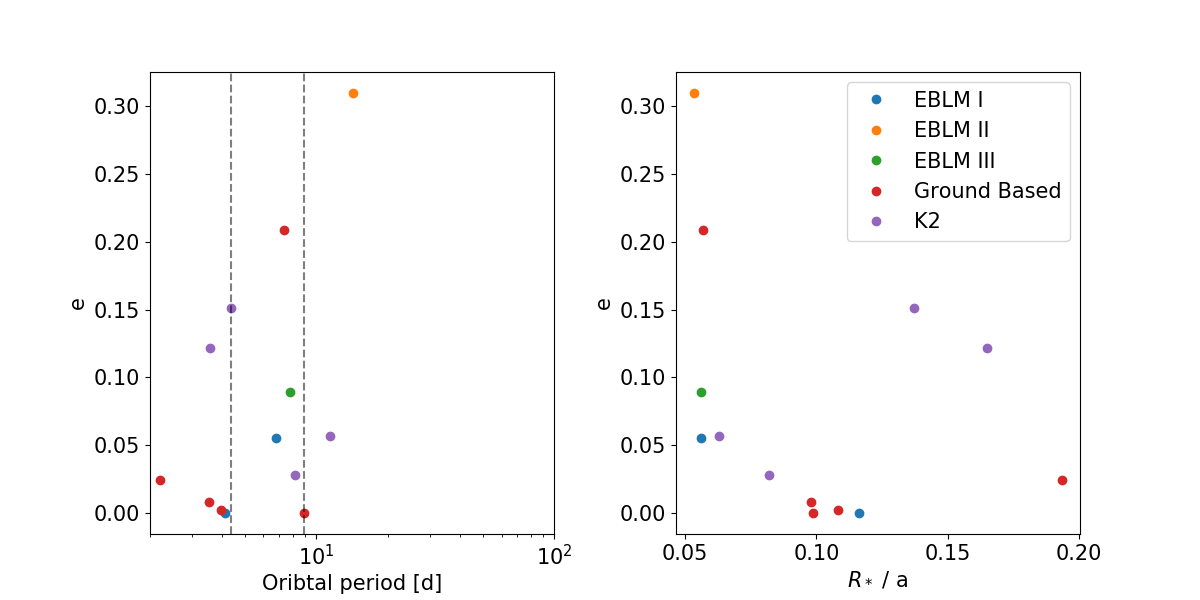
\includegraphics[width=\textwidth]{9-Discussion/images/tidal_trends_1.png}
    \caption{Eccentricity as a function of orbital period and scaled orbital separation. I report the EBLMs measured in the first three instalments of the EBLM project along with the nine EBLMs in this work.}
    \label{discussion:fig:tidal1}
\end{figure}

Eclipsing binary systems that have accurate measurements of masses, radii and rotation are can be used to probe the dynamical effects of tidal friction along with internal structure of each component. Probing the effects of tidal evolution requires measuring the degree of circularisation of the orbit and the level of synchronisation of the rotational velocities \citep{2010A&ARv..18...67T}. However, it is not easy to study the effects of tidal interactions as we are not able to follow the dynamical evolution of EBLMs from formation to the present. It is only possible to study those which we think formed with eccentric orbits that are now observed to circular, and make interpretations and conclusions which are not without questions. This is a very active field in which different prescriptions, theories and conclusions regarding tidal interactions are regularly exchanged (see \citet{2008EAS....29....1M} for an in-depth review). To the first approximation, tidal interactions reduce the eccentricity as a function of time such that,
%
\begin{equation}
    \frac{de}{dt} = -Ce,
\end{equation}
%
where the factor $C$ depends on the orbital separation, the internal structure of the two stars and their rotation \citep{2008EAS....29....1M}. The parameter $C$ usually varies on a timescale similar to the lifetime of the star and so is often assumed constant. In this case, the eccentricity decays exponentially,
%
\begin{equation}
    \frac{d\ln e}{dt} = \frac{1}{\tau_{\rm circ}}
\end{equation}
% 
where $\tau_{\rm circ}$ is the circularisation timescale. As shown in the seminal work by \citet{1975A&A....41..329Z}, $\tau_{\rm circ}$ is extremely dependent on the relative separation between stars,
%
\begin{equation}
    \tau_{\rm circ} \propto 
    \begin{cases}
    \left( \frac{a}{R_\star} \right)^8,  & \rm for \:\rm stars \:\rm with \: \textit{convective} \:\rm envelopes \\
    \left( \frac{a}{R_\star} \right)^{6.5},   & \rm for \:\rm stars \:\rm with \: \textit{radiative} \:\rm envelopes \\
    \end{cases}
\end{equation}
%
assuming negligible tidal dissipation in the secondary. Therefore EBLMs which have relatively tight orbits (high values of $R_\star / a$) and short periods are expected to have the smallest circularisation timescales, and thus all if not most of them should have a low eccentricity. In Fig. \ref{discussion:fig:tidal1} I plot eccentricity as a function period and $R_\star / a$ for all EBLMs measured within the scope of the EBLM project (including the nine reported in this work). The shorter period EBLM systems tend to have lower eccentricity although a significant number of long-period systems ($P_{\rm orb} = 5$--$10$\,d) also have low eccentricities. There appears to be no correlation with age. There is a clear decrease in eccentricity with scaled orbital separation indicating that stars with relatively compact orbits circularise more readily. There are two EBLM systems observed by K2 which deviate from this trend: (1) J0457$+$14 which is young and probably retained some primordial eccentricity and (2) J1652$-$19 which was noted to be relatively active akin to Kepler-17. 

There is some debate about the relevant timescale on which a systems orbit changes from eccentric or circular; this is called the transition period. To quote  \citet{2010A&ARv..18...67T},
%
\begin{quote}
``{\it Is the transition period the longest period for which a circular binary was found, or is it the shortest period with an eccentric orbit?}''
\end{quote}
%
Assuming a eccentricity upper-limit of $e < 0.05$, there are a six EBLMs of which the longest orbital period is 8.88\,d. For stars with $e > 0.05$, the shortest orbital period is 4.37\,d (excluding J0457$+$14). These ambiguous values exist for most data-sets and I have marked in Fig. \ref{discussion:fig:tidal1} to bound the possible range of the transition period.

\begin{figure}
    \centering
    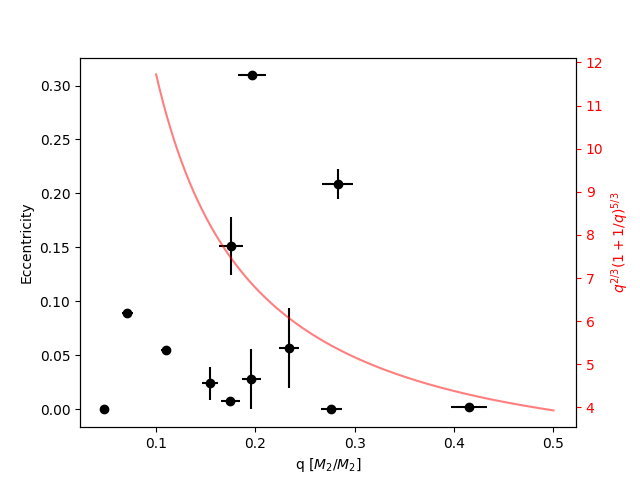
\includegraphics[width=\textwidth]{9-Discussion/images/tidal_trends_3.png}
    \caption{Eccentricity as a function of mass ratio, $q$, for all EBLMs measured within the EBLM project, and those measured in this work. We also show the predicted increase in $\tau_{\rm circ}$ found by \protect\citet{1988ApJ...326..256M}.}
    \label{discussion:fig:tidal3}
\end{figure}

The secondary mass can greatly influence the width of the transition region \citep{1988ApJ...326..256M}. The gravitational attraction of the M-dwarf companion is the source of the tidal force exerted on the primary star and so the circularisation timescale for the primary star is expected to be dependent on this value.  The dependency of $\tau_{\rm circ}$ with $q = M_2 / M_\star$ was explored by \citet{1988ApJ...326..256M} who found
%
\begin{equation}\label{discussion:t_circ_mass_ratio}
    \tau_{\rm circ} \propto q^{2/3}(1 + 1/q)^{5/3} .
\end{equation}
Therefore, the secondary mass can extend $\tau_{\rm circ}$  by a factor of 4, when moving from $q = 1$ to $q = 0.1$. I found no evidence that eccentricity correlated with mass ratio - see Fig.  \ref{discussion:fig:tidal3}. 

A final factor to account for is primordial eccentricity. A binary with initial eccentricity of 0.75 needs twice the amount of time needed by a binary with initial eccentricity of 0.2 to get to an eccentricity of 0.05 \citep{2010A&ARv..18...67T}. The youngest EBLM of the sample, J0457$+$14, has a smaller eccentricity than J1847$+$39 despite being ~400\,Myr older suggesting that J1847$+$39 could have formed with more primordial eccentricity. This may not be the case for J0457$+$39 which has a much larger value of $R_\star / a$ and would have experienced more intense tidal interaction than J1847$+$39. We need a much larger sample to pick out trends that may lie within the scatter produced by a range of primordial eccentricities.





\begin{figure}
    \centering
    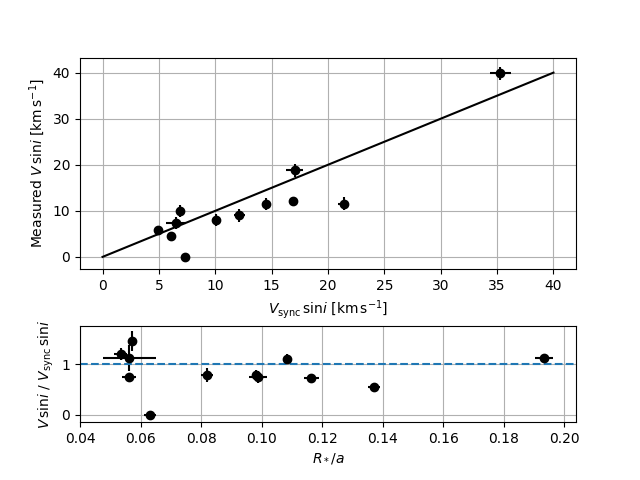
\includegraphics{9-Discussion/images/tidal_trends_2.png}
    \caption{Ratio between measured and projected (pseudo-)synchronous rotational velocities for EBLMs measured in the first three instalments of the EBLM project along with the nine EBLMs in this work (top panel). The ratio is also shown as a function of $R_\star / a$ (lower panel). }
    \label{discussion:fig:tidal2}
\end{figure}

Another quantity of importance is the synchronisation of companions in binary systems. Over an eccentric orbit, the tidal forces will be strongest at periastron and so the primar star is expected to rotate with an angular velocity between what is expected for field stars (i.e. from gyro-chronology) and the orbital angular velocity at periastron. The extent in which the primary star is spun up/down depends on the strength of the tidal interaction (i.e. $R_\star / a$). In Fig. \ref{discussion:fig:tidal2} shows the level of pseudo-synchronisation achieved by the stars as a function of $R_\star  /a$ (excluding J0457$+$14 for its youth and J0055$-$00 as I was unable to measure $V \sin i$). There are a distinct number of asynchronous stars with $R_\star / a < 0.08$ which is similar to the results found by \citet{2010A&ARv..18...67T} for systems with higher mass ratios. For stars with $R_\star / a > 0.08$, the majority of systems appear to be rotating slower than predicted for a synchronous orbit although this is likely an artefact of small-number statistics.










%	- Types of stars F/G and circularising/synchronisation%
%	- Is it expected? 
%	- Vsini predicted
%	- eccentricity distribution
%	- Everything in place to do it
%	- Do a M-R distribution plot compared to Torres (how does it depend on Mass ratio (q)
%		- What are the trends
%		- Scale with q
%	- tidal breaking contributn between M-dwarf and F type
%		 - check for each companion
%		- Do calculations to verify
		
		
		
		
		
		
		

		
		

		
\section{Selection effects}\label{discuss:selection}

I found that 4 out of 9 EBLM systems measured in this work has a primary star which has entered the ``blue-hook'' part of it's post main-sequence evolution. This occurs to stars in the mass range $1.1$--$1.5\,M_\odot$ which develop a small convective core during core hydrogen burning. Core hydrogen is depleted to the extent in which core fusion effectively stops, causing the star to contract and heat. In lower-mass stars ($\leq 1.1\,M_\odot$), the transition between core and shell hydrogen burning is gradual and so the star can remain in thermal equilibrium with an isothermal helium core. Stars which reside in or near the ``blue-hook'' part of it's post main-sequence evolution have some ambiguity surrounding mass and age. This ultimately leads to some ambiguity regarding which side of the ``blue-hook'' the primary star resides within leading to double peaked PPDs for $M_1$ and $\tau$. Ultimately, these systems are not suitable for empirical mass-radius calibrations as we cannot confidently break the mass degenercy using the host star. 

A solution is to turn EBLMs from single-lined eclipsing binaries to double-lined eclipsing binaries, where the masses can be directly measured. Achieving this is no easy feat which requires separation of atomic lines from the host star with molecular lines from the M-dwarf companion. The CORALIE \'{e}chelle spectrograph is unsuitable for this for two reasons: (1) the wavelength coverage is in the optical (300--750\,nm) where the contrast between the M-dwarf and the primary star is low and (2) a small telescope aperture does not permit the identification of otherwise faint molecular lines. The latter point can be addressed using the high SNR spectra obtained from SALT. I cross-correlated the red-arm spectra (560--870\,nm) for the EBLMs observed with SALT which are measured in this work (J2349$-$32, J2308$-$46, J0218$-$31 and J2217$-$04) with an M5 template provided through \textsc{ispec}. I failed to measure a radial velocity for the secondary component in all cases suggesting that a high SNR in the optical is not sufficient to overcome a low contrast ratio. In future work, I intend to acquire infrared spectra from such instruments as Long-slit Intermediate Resolution Infrared Spectrograph (LIRIS) on the 4.2-m William Herschel Telescope (0.9--2.4$\,\mu m$) or the Infra-Red Dual-beam Imager and Spectrograph (IRDIS) on the 8.2-m Very Large Telescope (VLT) where the contrast will be much larger than the optical. These observations will also provide an excellent test for evolutionary models of the host star from which the mass and age of the M-dwarf companion are derived from.

To avoid spending valuable follow-up time on EBLMs which have entered the ``blue-hook'' part of their post-main sequence evolution, I could select follow-up targets from a volume-limited sample of candidates.  Stars with masses below 1.1-$M_\odot$ do not exhibit a ``blue-hook'' phase in their evolution and so an obvious solution would be to follow-up stars with $T_{\rm eff} \lessapprox 5900$\,K. Selecting cooler stars has a number of drawbacks. First, there is an inherently low probability of G/K+M binaries surviving due to predictions from tidal interactions (Sec. \ref{introduction:EBLM}), and thus an inherently lower probability of finding such systems; only two out of nine systems presented here have primary star temperatures below . 5900\,K. Secondly, cooler primary stars result in higher ratios of $R_2/ R_1$ ($k$), leading to a higher chance of a transit being grazing in nature ($b > 1$), or such that the radius of the two components cannot be accurately determined (such as J1436$-$13 or J0055$-$00). The second data release of Gaia provides some indication regarding the evolutionary status of the primary star in EBLM systems. A future vetting procedure may involve selecting those with colours consistent with dwarf-like surface. 

The EBLMs used in this work were identified by the WASP survey and so are subjected to selection biases. Querying \textsc{tepcat} \citep{2011MNRAS.417.2166S}\footnote{http://www.astro.keele.ac.uk/jkt/tepcat/, accessed 1 Oct 2018} reveals that there are 157 WASP exoplanet systems. Exactly half of the host stars have surface temperatures measured to be below 5900\,K and have a broad metallicty peak around $+0.1$\,dex. A query of the WASP database\footnote{accessed 1 Oct 2018} yields 926 systems flagged as ``EBLM''.  Of those, 455 (48\%) have IRFM temperatures below 5900\,K.

%and only 144 reside near or within the main sequence in the $G$-($G_{\rm rp} - G_{\rm bp}$)\footnote{selected by inspection} plane.

The field of eclipsing binaries and exoplanets is gently transitioning from an era of detection to an era of characterisation. Large quantities of data exist from numerous ground-based surveys and current/forthcoming space observatories. To a measure the masses, radii and ages of EBLMs reliably requires a diligent screening of potential EBLM systems. Even with the volume limited sample ($T_{\rm eff} < 5900$ and using Gaia DR2) we still have over 140 EBLMs which could be suitable to be measured withing the EBLM project. A significant portion of these will be false-positives, blended EBs, or have unfavourable transit geometries (e.g. high impact parameters). However, we only follow-up EBLMs if we detect the primary eclipse which is more likely for bigger M-dwarfs around smaller stars. This will lead to a bias in the mass-radius diagram which will need accounting for when the absolute parameters of more EBLMs are determined. 

%There will still be a significant amount of of systems remaining for which measurements of masses and radii can be achieved with an uncertainty of a few percent and contribute to empirical calibrations.

	
\section{GP-GPU lightcurve model}\label{discussion:qpower2}

%There is a large selection of well-tested and reliable software tools to study eclipsing binary systems. The fast and flexible lightcurve model \textsc{ellc} models stars as tri-axial ellipsoids to create an eclipsing-binary model which can include the effects of star spots, Doppler boosting and light-travel time for binary stars. The lightcurve model \textsc{jktebop} \citep{2013A&A...557A.119S} is a \textsc{fortran} implementation of the Eclipsing Binary Orbit Program (\textsc{ebop}; \citealt{1993IAUCB..21..113E}) which treats stars as spherical for eclipse shapes and bi-axial spheroids for reflection and ellipsoidal effects. The Bad-Ass Transit Model cAlculatioN (\textsc{batman}; \citealt{2015PASP..127.1161K}) is an $C$-powered exoplanet transit model  with a python interface. \textsc{batman} provides parallelisation at the C-level with \textsc{openmp}$\textregistered$ \citep{Dagum:1998:OIA:615255.615542} and is capable of calculating a million model light curves in well under 10 minutes for any limb darkening profile\footnote{www.cfa.harvard.edu/~lkreidberg/batman}. 

The increase in CPU clock rates lead to an increase in execution speeds of lightcurve models until the early 2000's. Since then increase in CPU clock rates has stalled as CPU manufactures struggled to dissipate the heat from faster chip-sets (\citealt{2018arXiv181006250S}; \citealt{patterson2014computer}). Graphic proccessing units (GPUs) extend this idea by maximising the number of cores on a chip. The GTX 1080 used in this work has 2,560 processing cores divided up onto 20 streaming micro-processors.  While GPUs were originally desinged to be used as graphical processors to handle resolution, display rates and ray-tracing demanded by the videogame industry, the computing cabability has been exploited leading to general-purpose GPU (GP-GPU) programs such as projects in artificial intelligence (e.g. \citet{2017SPIE10454E..06B}) and deep learning (e.g. \citet{2018arXiv180404806O}). A review of GPU use in scientific computing can be found in \citet{Owens2007} and \citet{Owens2008}.



My implementation of the \textsc{qpower2} model is written in $C$ using \textsc{CUDA}\textregistered  toolkit V10.0\footnote{https://developer.nvidia.com} provided by \textsc{NVIDIA}\textregistered and has a python front-end. It supports \textsc{OpenMP}\textregistered  which permits efficient multiprocessing. When determining the orbital solution, it is more efficient to use a single processor per model and evaluate multiple models for each ``step'' in parallel. This is a feature offered within \textsc{emcee} and each call to \textsc{qpower2} is thread safe. Manafactures work around the \textit{thermal-wall} by implementing multiple processors on a single chip achieving a higher throughput through parallelisation. 

\begin{figure}
    \centering
    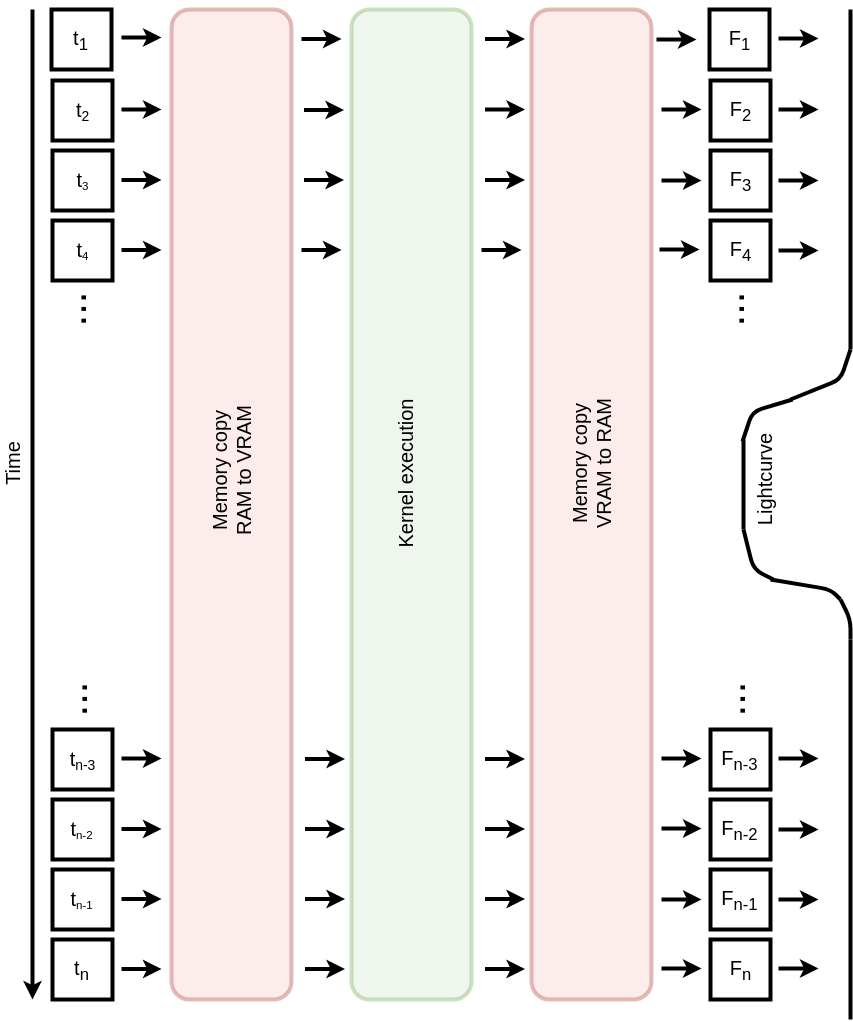
\includegraphics[width = \textwidth]{9-Discussion/images/GPU_execution_1.png}
    \caption{The sequence of execution when calculating a lightcurve model on the GPU. The time sequence is represented by time stamps, $t_i$, and the respective flux, $F_i$.  }
    \label{discussion:fig:GPU_execution_1}
\end{figure}


\begin{sidewaystable*}[]
    \centering
    \caption{Execution times for the analytical \textsc{qpower2} model for a typical Kepler/K2 lightcurve and ground-based lightcurve. We assume a planet with $k=0.1$.}
    \label{discussion:tab:qpower2_timings}
    \begin{tabular}{l c l l c}
    \hline
    \hline

     Algorithm & Processor & Single model & Models /s & Notes \\
     \hline
     
     
     Hardware \\
    \multicolumn{4}{l}{Intel\textregistered Core\textsuperscript{TM} i7-7700K CPU 4.20\,GHz × 8 (overclocked to 4.8 GHz)} \\
    \multicolumn{3}{l}{GeForce GTX\textsuperscript{TM} 1080 (/PCIe/SSE2)} \\  Ubuntu 17.10 \\

    \hline
     \multicolumn{3}{l}{Kepler lightcurve (3840 time stamps)}\\
     \textsc{qpower2} (CPU) & 4.8\,GHz CPU & $357\,\mu s$ & 2801  \\
     \textsc{qpower2} (CPU) & 4.8\,GHz CPU$\times 8$ & $112\,\mu s$ & 8928 & Using OpenMP\textregistered   \\
     \textsc{qpower2} (GPU) & GTX 1080 & $228\,\mu s$ & 4385   \\
     \textsc{qpower2} (GPU) & GTX 1080 & $13\,\mu s$ & 75,851 & Computing 10,240 lightcurves    \\
     \textsc{qpower2} (GPU) & GTX 1080 & $2\,\mu s$ & 390,839 & Computing 10,240 lightcurves,    \\
     & & & & returning only $\mathcal{L}$\\
    \hline
    \multicolumn{3}{l}{SAAO light curve (345 time stamps)}\\
     \textsc{qpower2} (CPU) & 4.8\,GHz CPU & $50\,\mu s$ & 20,80  \\
     \textsc{qpower2} (CPU) & 4.8\,GHz CPU$\times 8$ & $21\,\mu s$ & 48,780 & Using OpenMP\textregistered   \\
     \textsc{qpower2} (GPU) & GTX 1080 & $12\,\mu s$ & 83,334   \\
     \textsc{qpower2} (GPU) & GTX 1080 & $1.3\,\mu s$ & 753,012 & Computing 10,240 lightcurves    \\
     \textsc{qpower2} (GPU) & GTX 1080 & 4.52\,ns & 2,211,900 & Computing 10,240 lightcurves,    \\
     & & & & returning only $\mathcal{L}$\\
    \hline 
    
    
    \end{tabular}
\end{sidewaystable*}

The four EBLMs measured using \textsc{qpower2} were called using code which executes on the CPU. A significant decrease in computational time can be achieved when this is executed on a graphics processing unit (GPU) instead instead. Various lightcurve models include support for GPUs; these include \textsc{batman}, \textsc{ExofastGPU} (an extension of \textsc{Exofast} for the GPU; \citealt{017ascl.soft10003E}) and \textsc{pytransit} \citep{2015MNRAS.450.3233P}. These implementations operate in a way similar to \textsc{OpenMP}\textregistered for CPU code; each time stamp is modelled using a single microprocessor on the GPU. The clock-speed (i.e. how fast calculations can be done) for GPU microprocessors is typically between 1-2\,GHz and is not far below the speed of a typical CPU processor (2-5\,GHz) and permits fast and efficient lightcurve synthesis. A major drawback is that GPUs are separate devices which connect to a motherboard through a principle component interconnect (PCI), and thus require costly memory transfer operations between the random access memory (RAM) and videocard random access memory (VRAM). The computational gain from GPU lightcurve synthesis is often quashed by memory transfer operations of the time axis and the resulting lightcurve (Fig. \ref{discussion:fig:GPU_execution_1}). This can be demonstrated with the \textsc{qpower2} model; calculating a lightcurve model for K2 lightcurve (~4000 time stamps) takes approximately $357\,\mu s$ on the CPU and $228\,\mu s$ on the GPU ($\sim 30\%$ speed increase; see Table \ref{discussion:tab:qpower2_timings} ). 

\begin{figure}
    \centering
    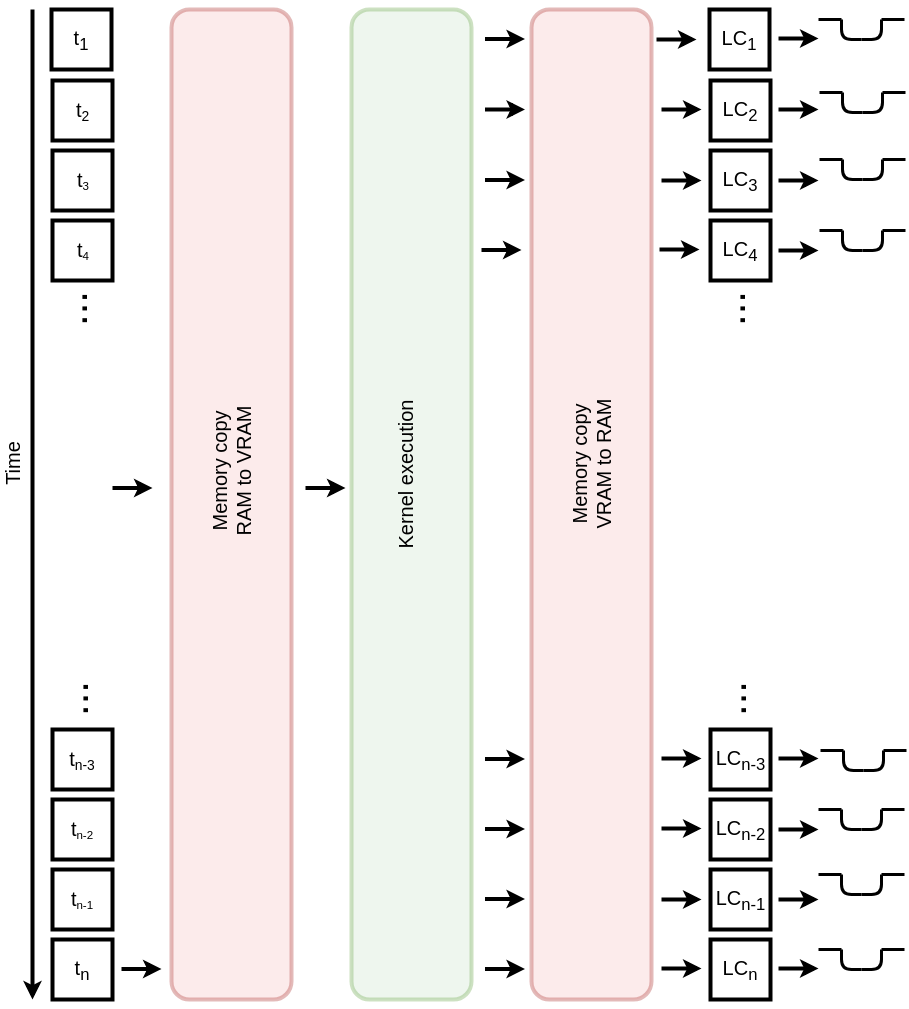
\includegraphics[width = \textwidth]{9-Discussion/images/GPU_execution_2.png}
    \caption{The sequence of execution when calculating many lightcurve models on the GPU. The time sequence is represented by time stamps, $t_i$, and the respective lightcurve model, $LC_i$.  }
    \label{discussion:fig:GPU_execution_2}
\end{figure}

Generating a single lightcurve model is therefore inefficient due to memory transfer operations. A better approach is to generate thousands of models at once and initiate a single memory transfer back to the host (Fig. \ref{discussion:fig:GPU_execution_2}). This method offers a significant speed-up as only one memory transfer operation is called. This method benefits users wishing to fit lightcurves with Bayesian methods that require multiple ``walkers'' (such as \textsc{emcee}). In this case, I chose to calculate 10,240 models at once ($2560$ micro-processors $\times 4$) which corresponds to a $60\times$ speed-up than the fastest CPU implementation.  

If fitting light-curves is the goal, then the only quantity of interest is the log-likelihood, $\mathcal{L}$.  A further optimisation can be achieved by returning only $\mathcal{L}$ for each model, rather than the entire model itself. This implementation offers a further $\times 8$ speed-up and  highlights the expense of memory transfer operations.

Using the GPU to only return $\mathcal{L}$ significantly accelerates Bayesian fitting routines; I am now able to initialise 10,240 ``walkers'' to explore parameter space. The architecture of the parallel-stretch move algorithm is such that convergence benefits from a large number of walkers, resulting in faster convergence and more reasonable acceptance fractions. To implement this, I modified the source code for \textsc{emcee} to accept an array of $\mathcal{L}$ for each ``step'' in Bayesian analysis. For a typical K2 lightcurve, I was able to sample 2 million draws is less 10 seconds; there is a small overhead checking the bounds of each trial step which is done on the CPU. Relevant parts of the code are presented in Appendix \ref{appendix:qpower2}.

In Sect. \ref{method:orbital_fit}, we used Gaussian processes to account for red noise in the K2 lightcurves. Conventional Gaussian processes requires an $n^2$ covariance matrix for a lightcurve with length $n$. Memory quickly becomes an issue when 10,240 $n \times n$ matrices are required to batch-compute red-noise models on the GPU. The package \textsc{celerite} used in Sect. \ref{methods:rednoise} cleverly reduces this dependency to an array of length $n$ from which to calculate a red-noise model. However, the dependencies of \textsc{celerite} are not GPU compatible and I am actively seeking a solution. The capability to generate thousands of lightcurve models on the GPU with a red-noise model will be an incredible powerful tool to analyse data from a variety of upcoming space-based missions. 
